% !TeX root = ../main.tex

\chapter{Related Work}
\label{ch:relWork}
Since the introduction of the smartphone, taking images of food has become much more appealing for many people. There is an increasing trend to share images of food on social media. Since people get used to taking pictures of their food, images have become a much more interesting approach for data collection. Following this trend there is an growing number of publications in the field of food recognition. The goal of this chapter is to provide an overview of the key aspects of this field such as available datasets, common algorithms and existing systems.

\section{Datasets}
\label{sec:relWork_Datasets}
Comprehensive datasets are an important requirement for any modern image recognition task. For non-food objects like planes, animals or plants there are many huge, high-quality datasets with a sufficient amount of data such as ImageNet \cite{Russakovsky2015} or CIFAR-10 \cite{Krizhevsky2009}. Since computer vision algorithms for food classification have to deal with more intra-class-variance {(see Section \ref{sec:introduction_challenges})} datasets have to be sufficiently big to be able to train accurate models. However, most of the existing food recognition datasets tend to be to small, have to much noise {(false labels)} or contain only images in controlled environments. Another problem that datasets are not able to cover so far is the high number of different classes for food. So even if a dataset covers 100 various types of meals this is still only a small amount compared to the number of actual food-recipes. The following section and table~\ref{tab:datasetsComparison} will give a brief overview and comparison of datasets usable for food recognition.

\begin{table}[htbp]
	\centering
	\begin{tabular}{@{}lrrll@{}}
		\toprule
		\multicolumn{1}{c}{\textbf{Name}} & \multicolumn{1}{c}{\textbf{\# Classes}} & \multicolumn{1}{c}{\textbf{\# Images}} & \multicolumn{1}{c}{\textbf{Source}} & \multicolumn{1}{c}{\textbf{Comments}} \\ \midrule
		\hyperref[subsec:relWork_Datasets_food101]{ETHZ-Food-101}                    & 101                                     & 101000                                 & \cite{Bossard2014}                              &                                       \\
		\hyperref[subsec:relWork_Datasets_food101]{UPMC Food-101}                     & 101                                     & 101000                                 & \cite{Kumar2015}                              &                                       \\
		
		\hyperref[subsec:relWork_Datasets_food201]{Food201-MultiLabel}                & 201                                     & 47374                                  & \cite{Meyers2015}                              & to be released                        \\
	
		\hyperref[subsec:relWork_Datasets_food100256]{UEC Food 256}                      & 256                                     & 31651                                  & \cite{Kawano2015}                              &                                       \\
	
		\hyperref[subsec:relWork_Datasets_food201]{Food201-Segmented}                 & 201                                     & 12625                                  & \cite{Meyers2015}                              & to be released                        \\
		
		\hyperref[subsec:relWork_Datasets_food100256]{UEC Food 100}                      & 100                                     & 9060                                   & \cite{Matsuda2012}                              &                                       \\
		
		50-data							  & 50                                      & 5000                                   & \cite{Chen2012}                              &                                       \\
		
		\hyperref[subsec:relWork_Datasets_pfid]{PFID}                              & 7                                     & 4545                                   & \cite{Chen2009}                              & 101 different foods                                      \\
		
		\hyperref[subsec:relWork_Datasets_menuMatch]{Menu-Match}                              & 41                                     & 646                                   & \cite{Beijbom2015}                              & includes calorie count                                      \\
	
	\end{tabular}
	\caption{Comparison of publicly available datasets for food classification.}
	\label{tab:datasetsComparison}
\end{table}

\subsection[PFID]{Pittsburgh Fast Food Image Dataset}
\label{subsec:relWork_Datasets_pfid}
In 2009 Chen et al. released the first publicly available\footnote{\texttt{http://pfid.rit.albany.edu/index.php}, accessed 2016-03-02} food dataset also known as the \gls{pfid} \cite{Chen2009}. They collected food from eleven fast food chains popular in the \gls{usa}, then selected 101 different foods from these restaurants and took 4,545 still images in both controlled laboratory conditions and in the restaurants itself. Each restaurant was visited at least three times on different dates to get varying instances of the same food. For the still images in the lab they took six pictures of each item on a rotating turntable with each picture being 60 degrees apart. The images in the restaurant were taken with and without wrapper and from all four sides resulting in 8 images in the restaurant setting and 6 in the controlled environment per food and instance. In addition, they also took 606 stereo images {(one or two for each food)}, a 360 degree video of the item on the turntable and 27 videos of people eating the food. Since their recognition rate for the 101 classes was very low they combined the 101 different items into seven more abstract categories as seen in figure~\ref{fig:pfidExamples}. The \gls{pfid} focuses on fast food because it is highly standardised {(the food looks similar even across different restaurants)} and a key factor for obesity. For these reasons many publications use this dataset to benchmark their models.
\begin{figure}[htbp]
	\centering
	\subfloat[sandwiches, subs, wraps]{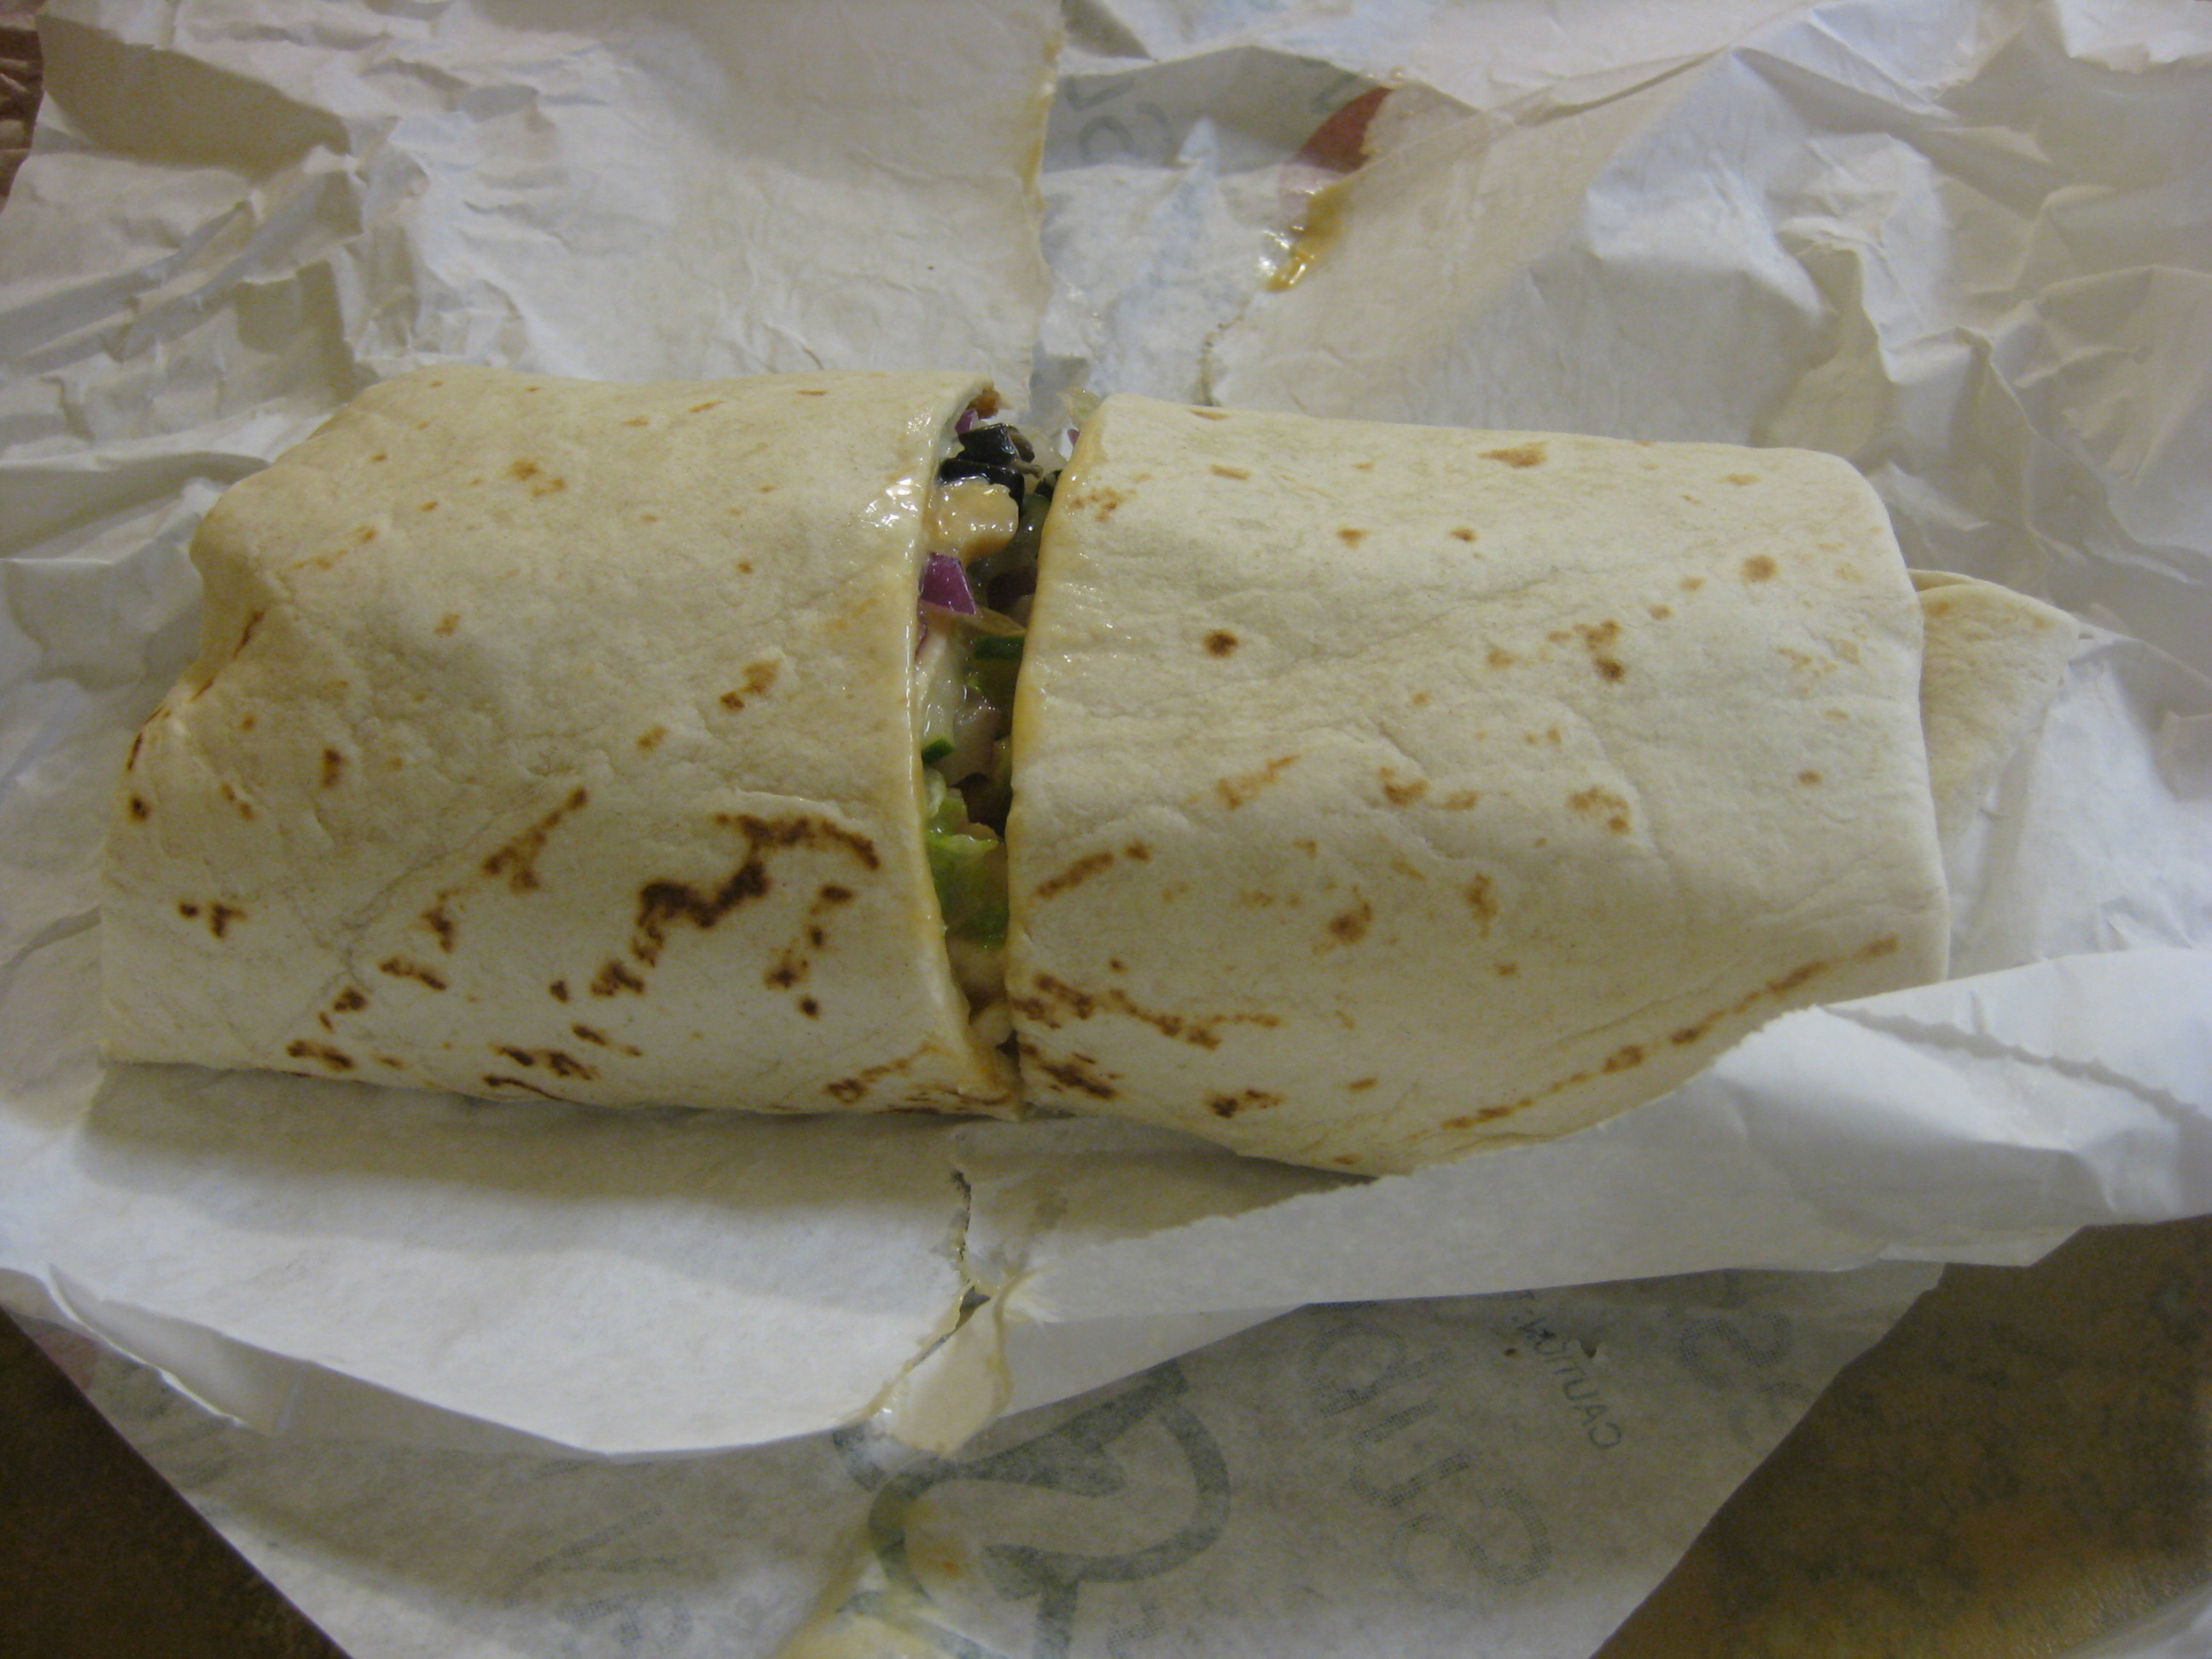
\includegraphics[width=20mm]{data/images/relWork/pfid_sandwich}}
	\subfloat[meat]{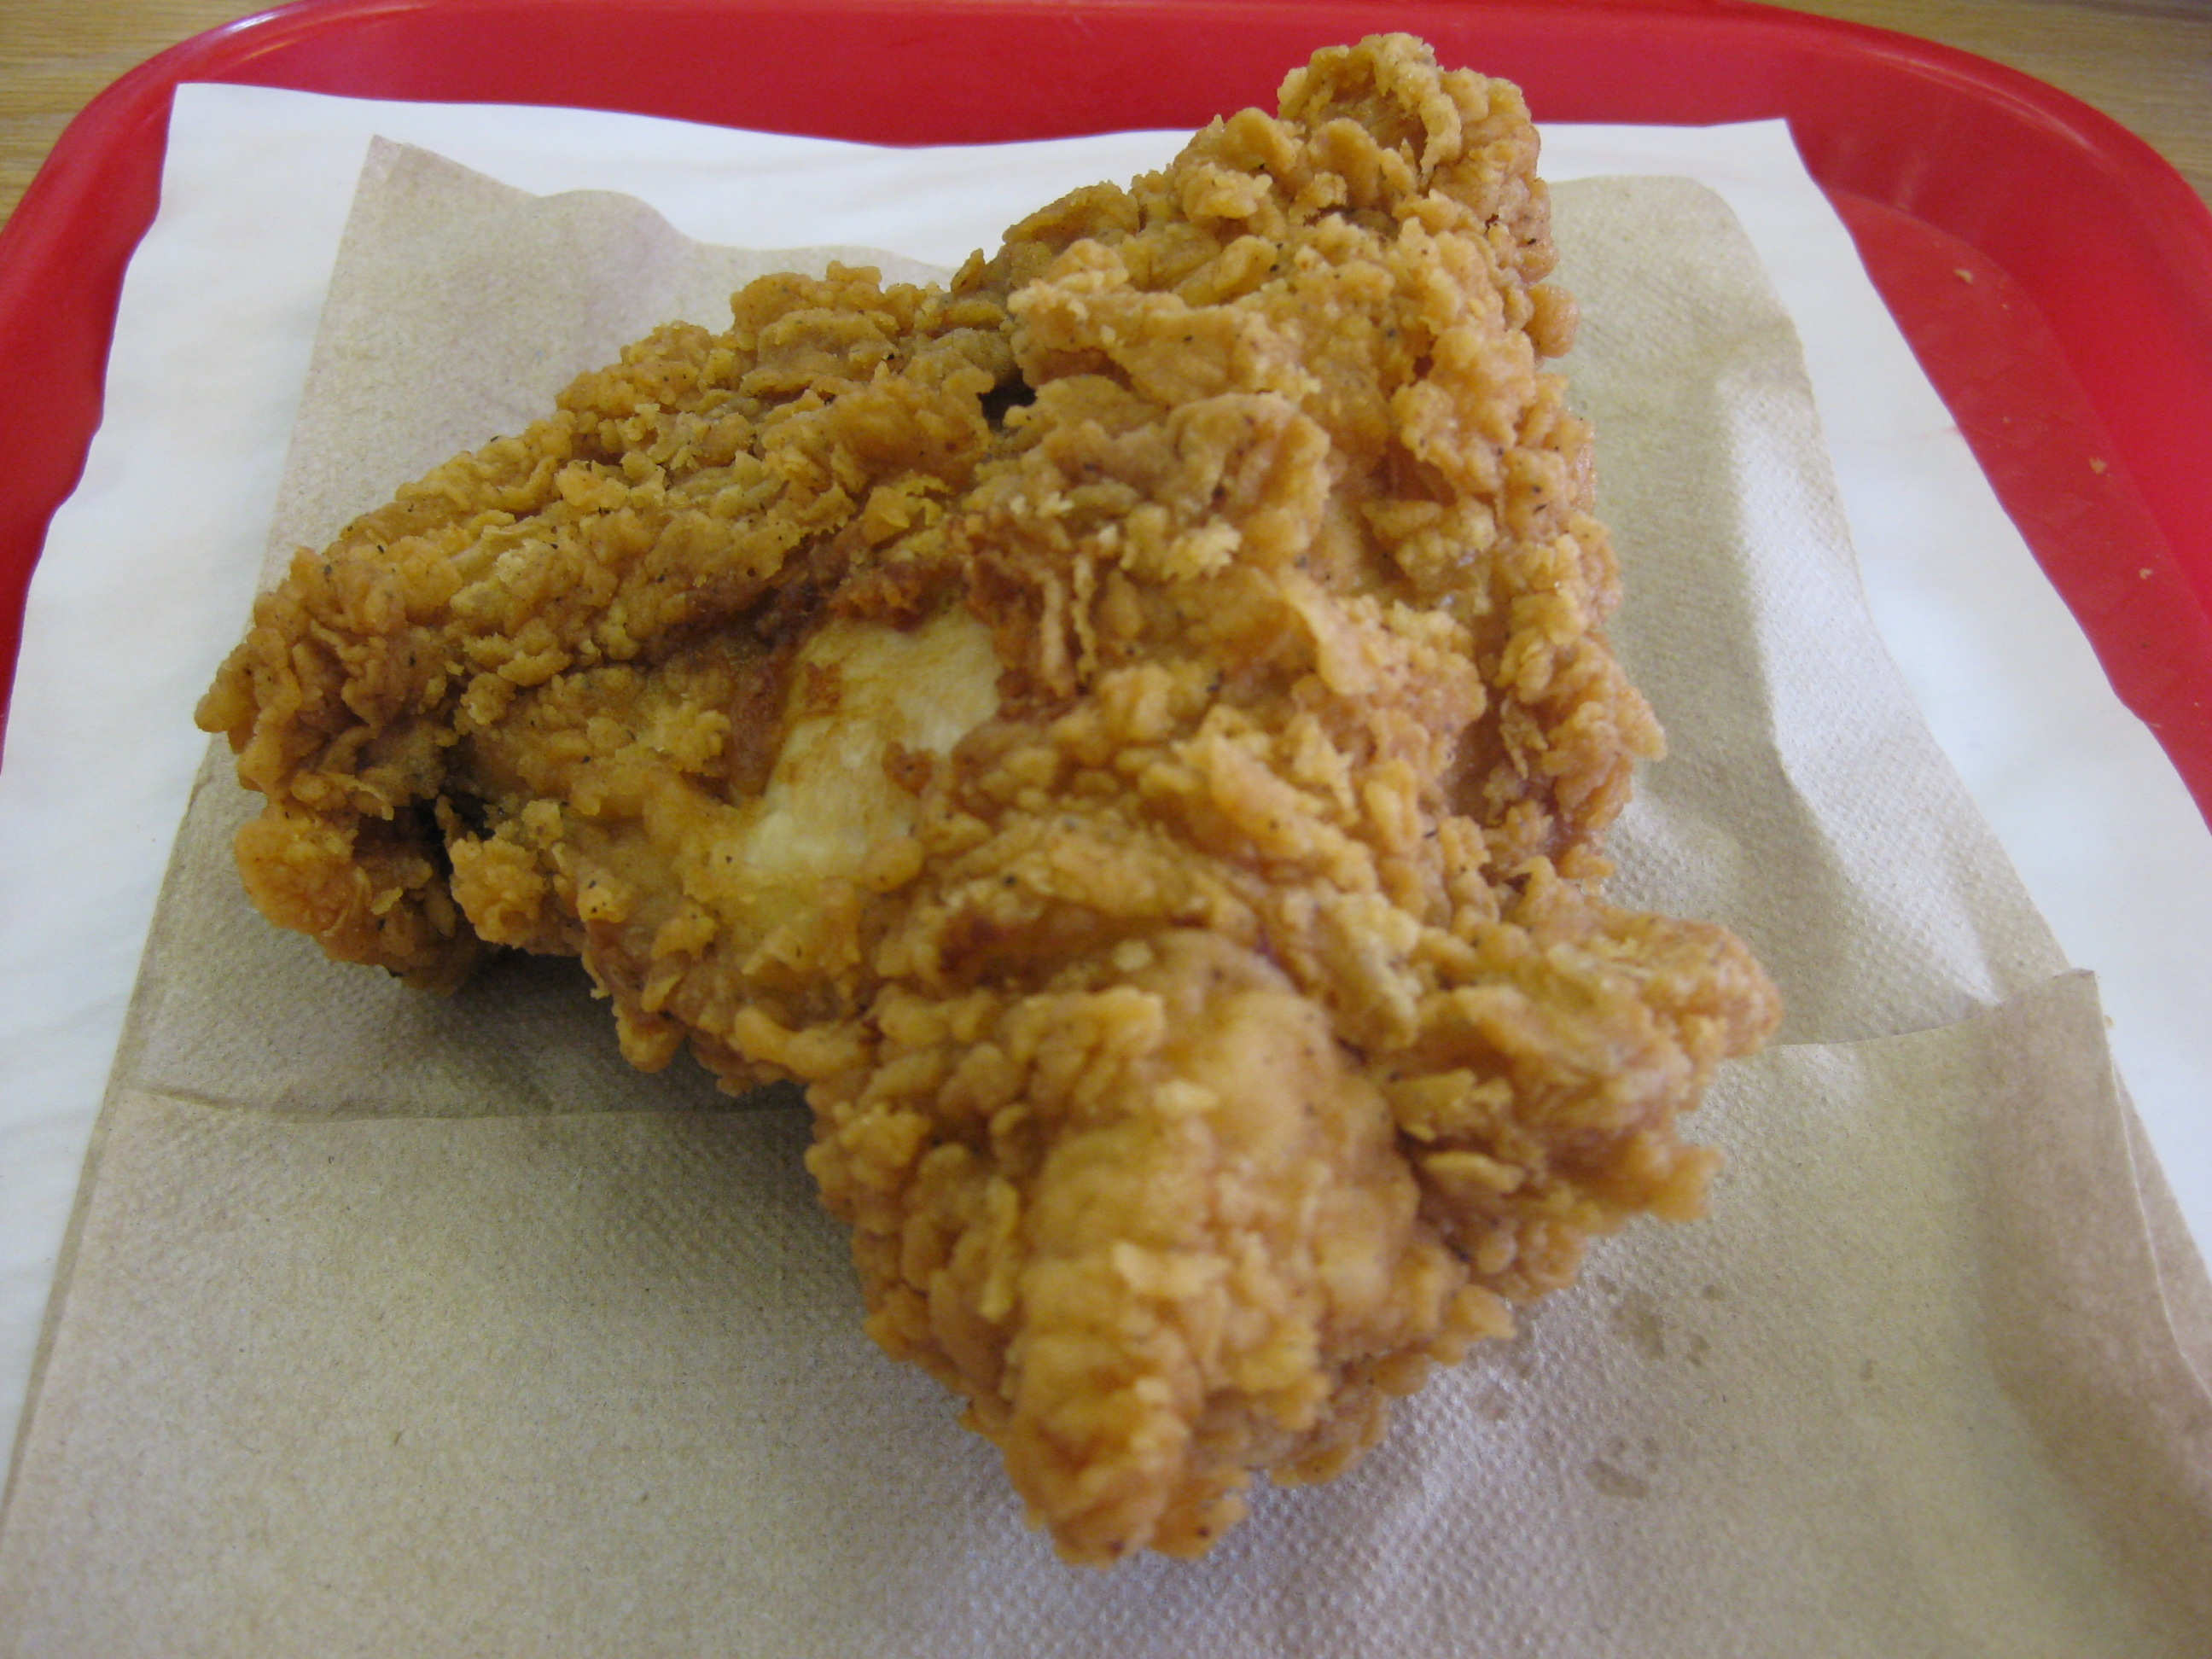
\includegraphics[width=20mm]{data/images/relWork/pfid_miscMeat}}
	\subfloat[salads]{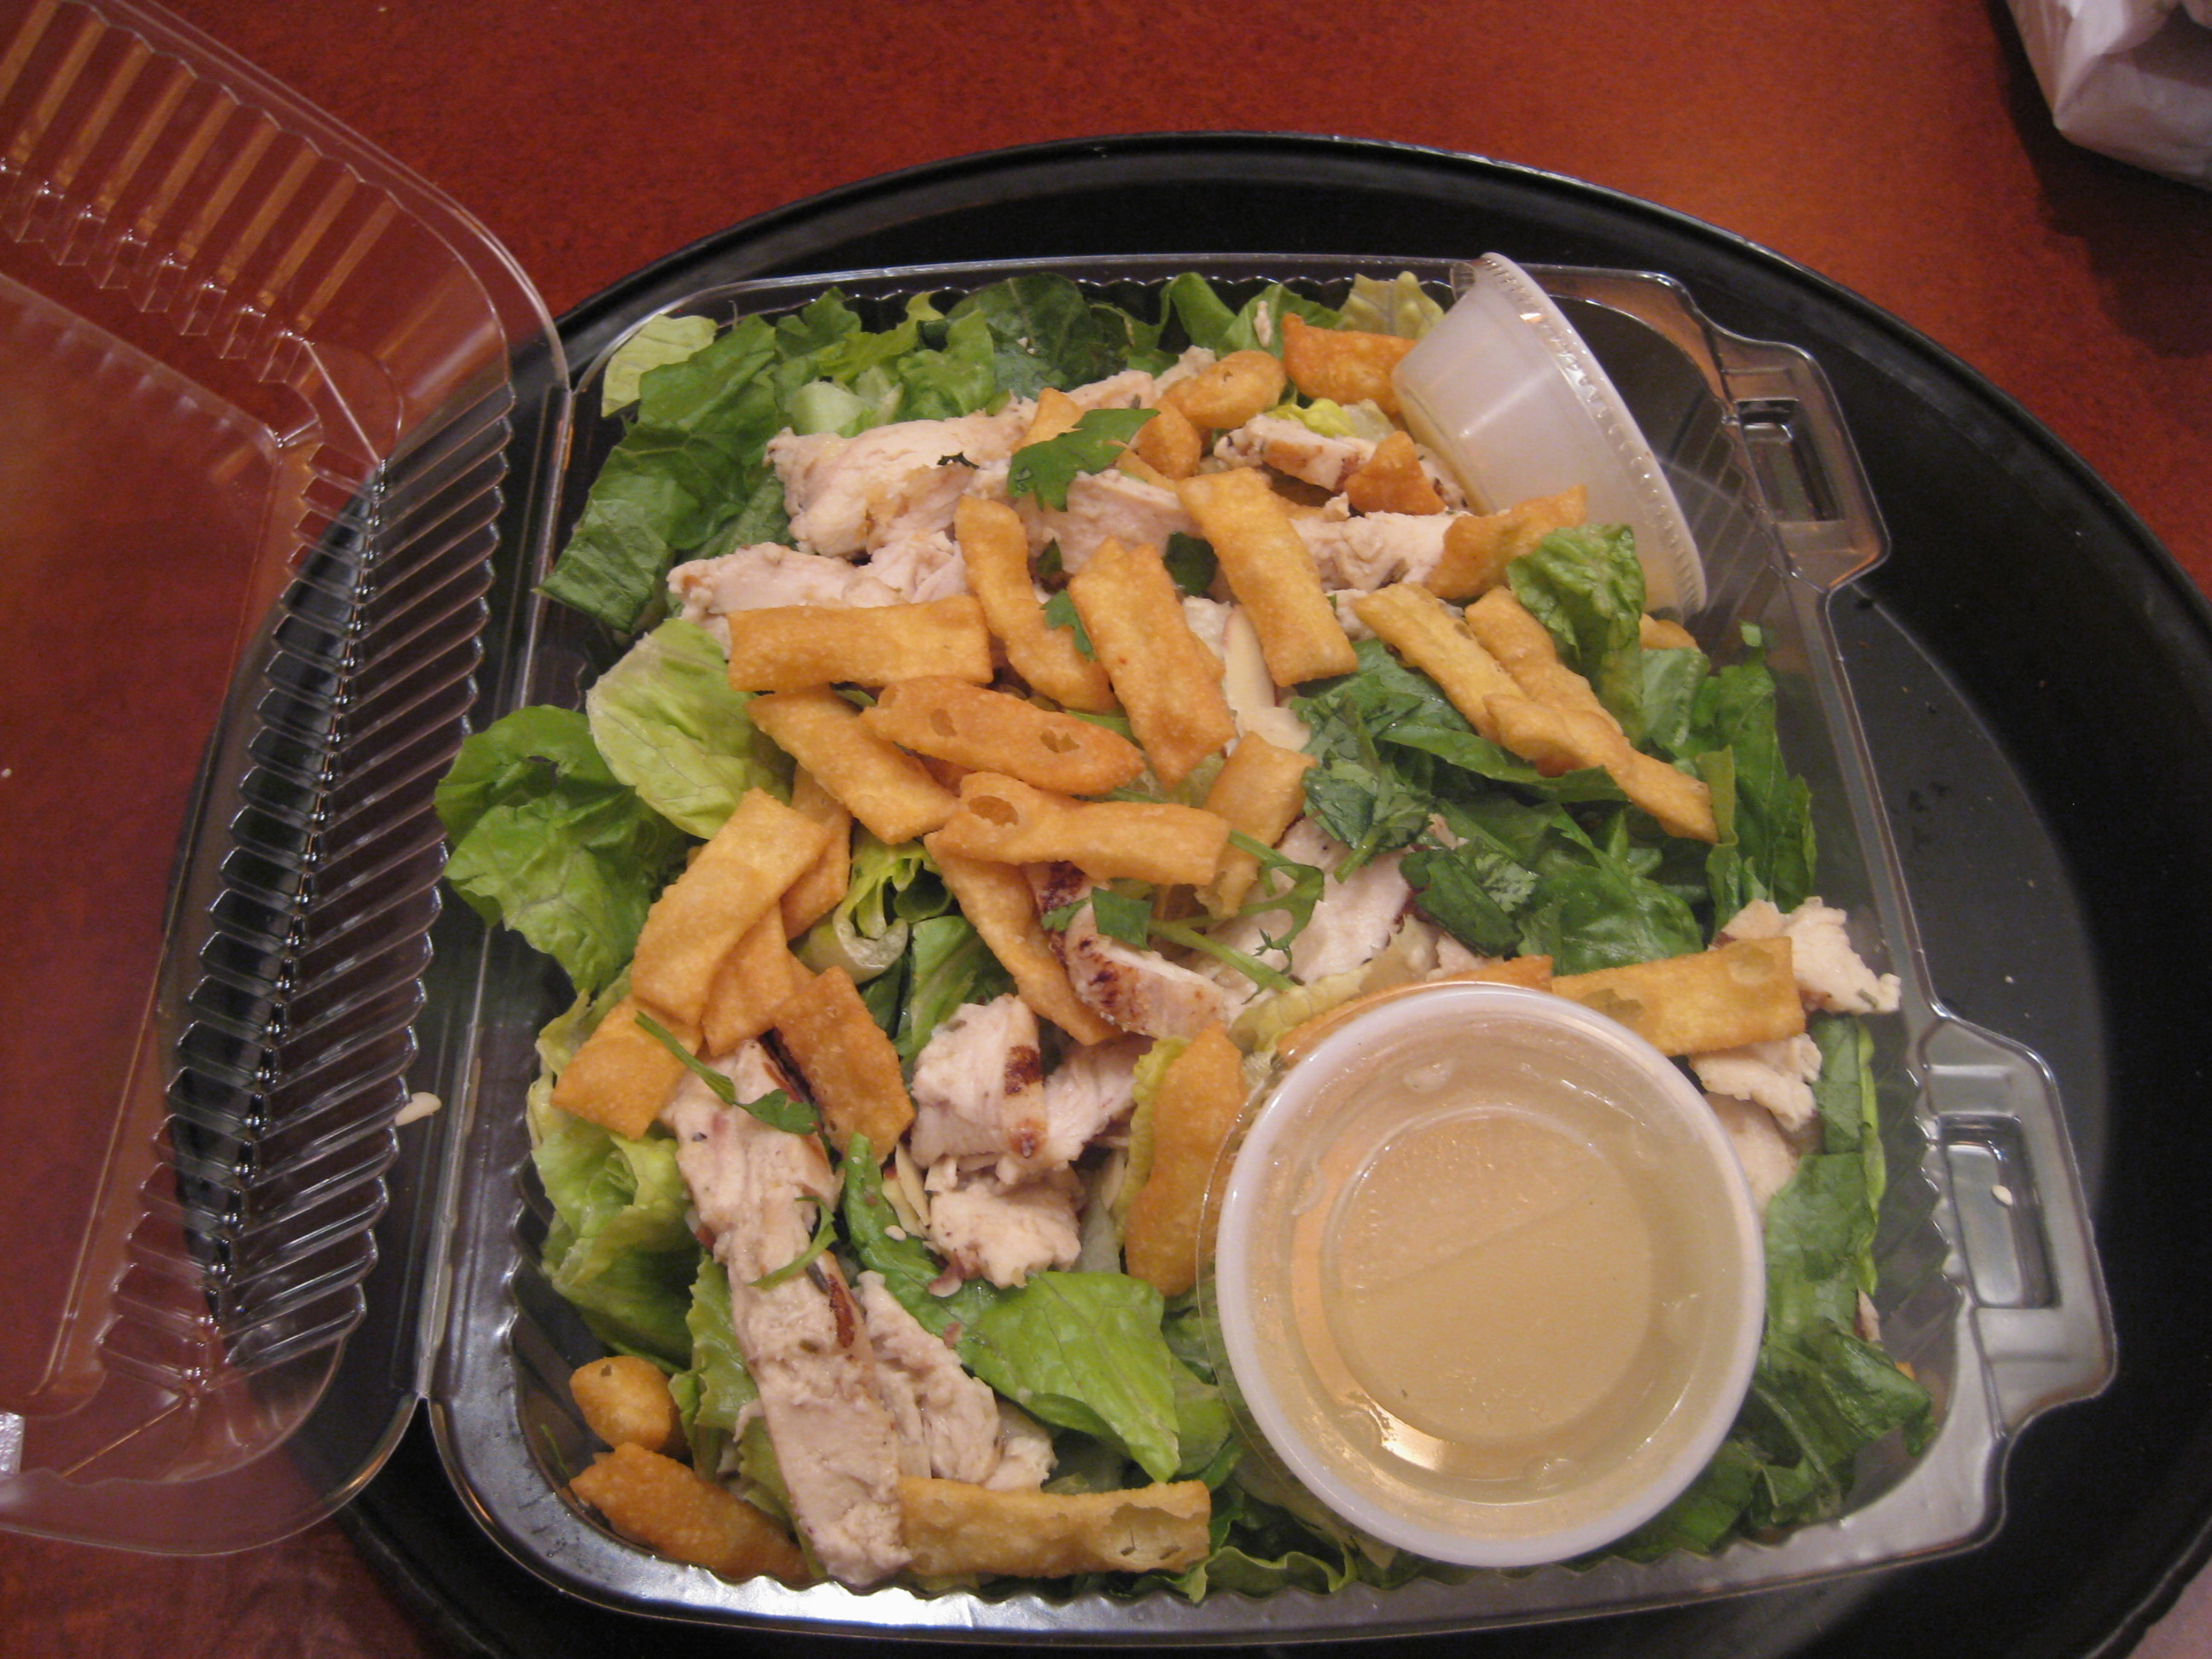
\includegraphics[width=20mm]{data/images/relWork/pfid_salad}}
	\subfloat[bagels]{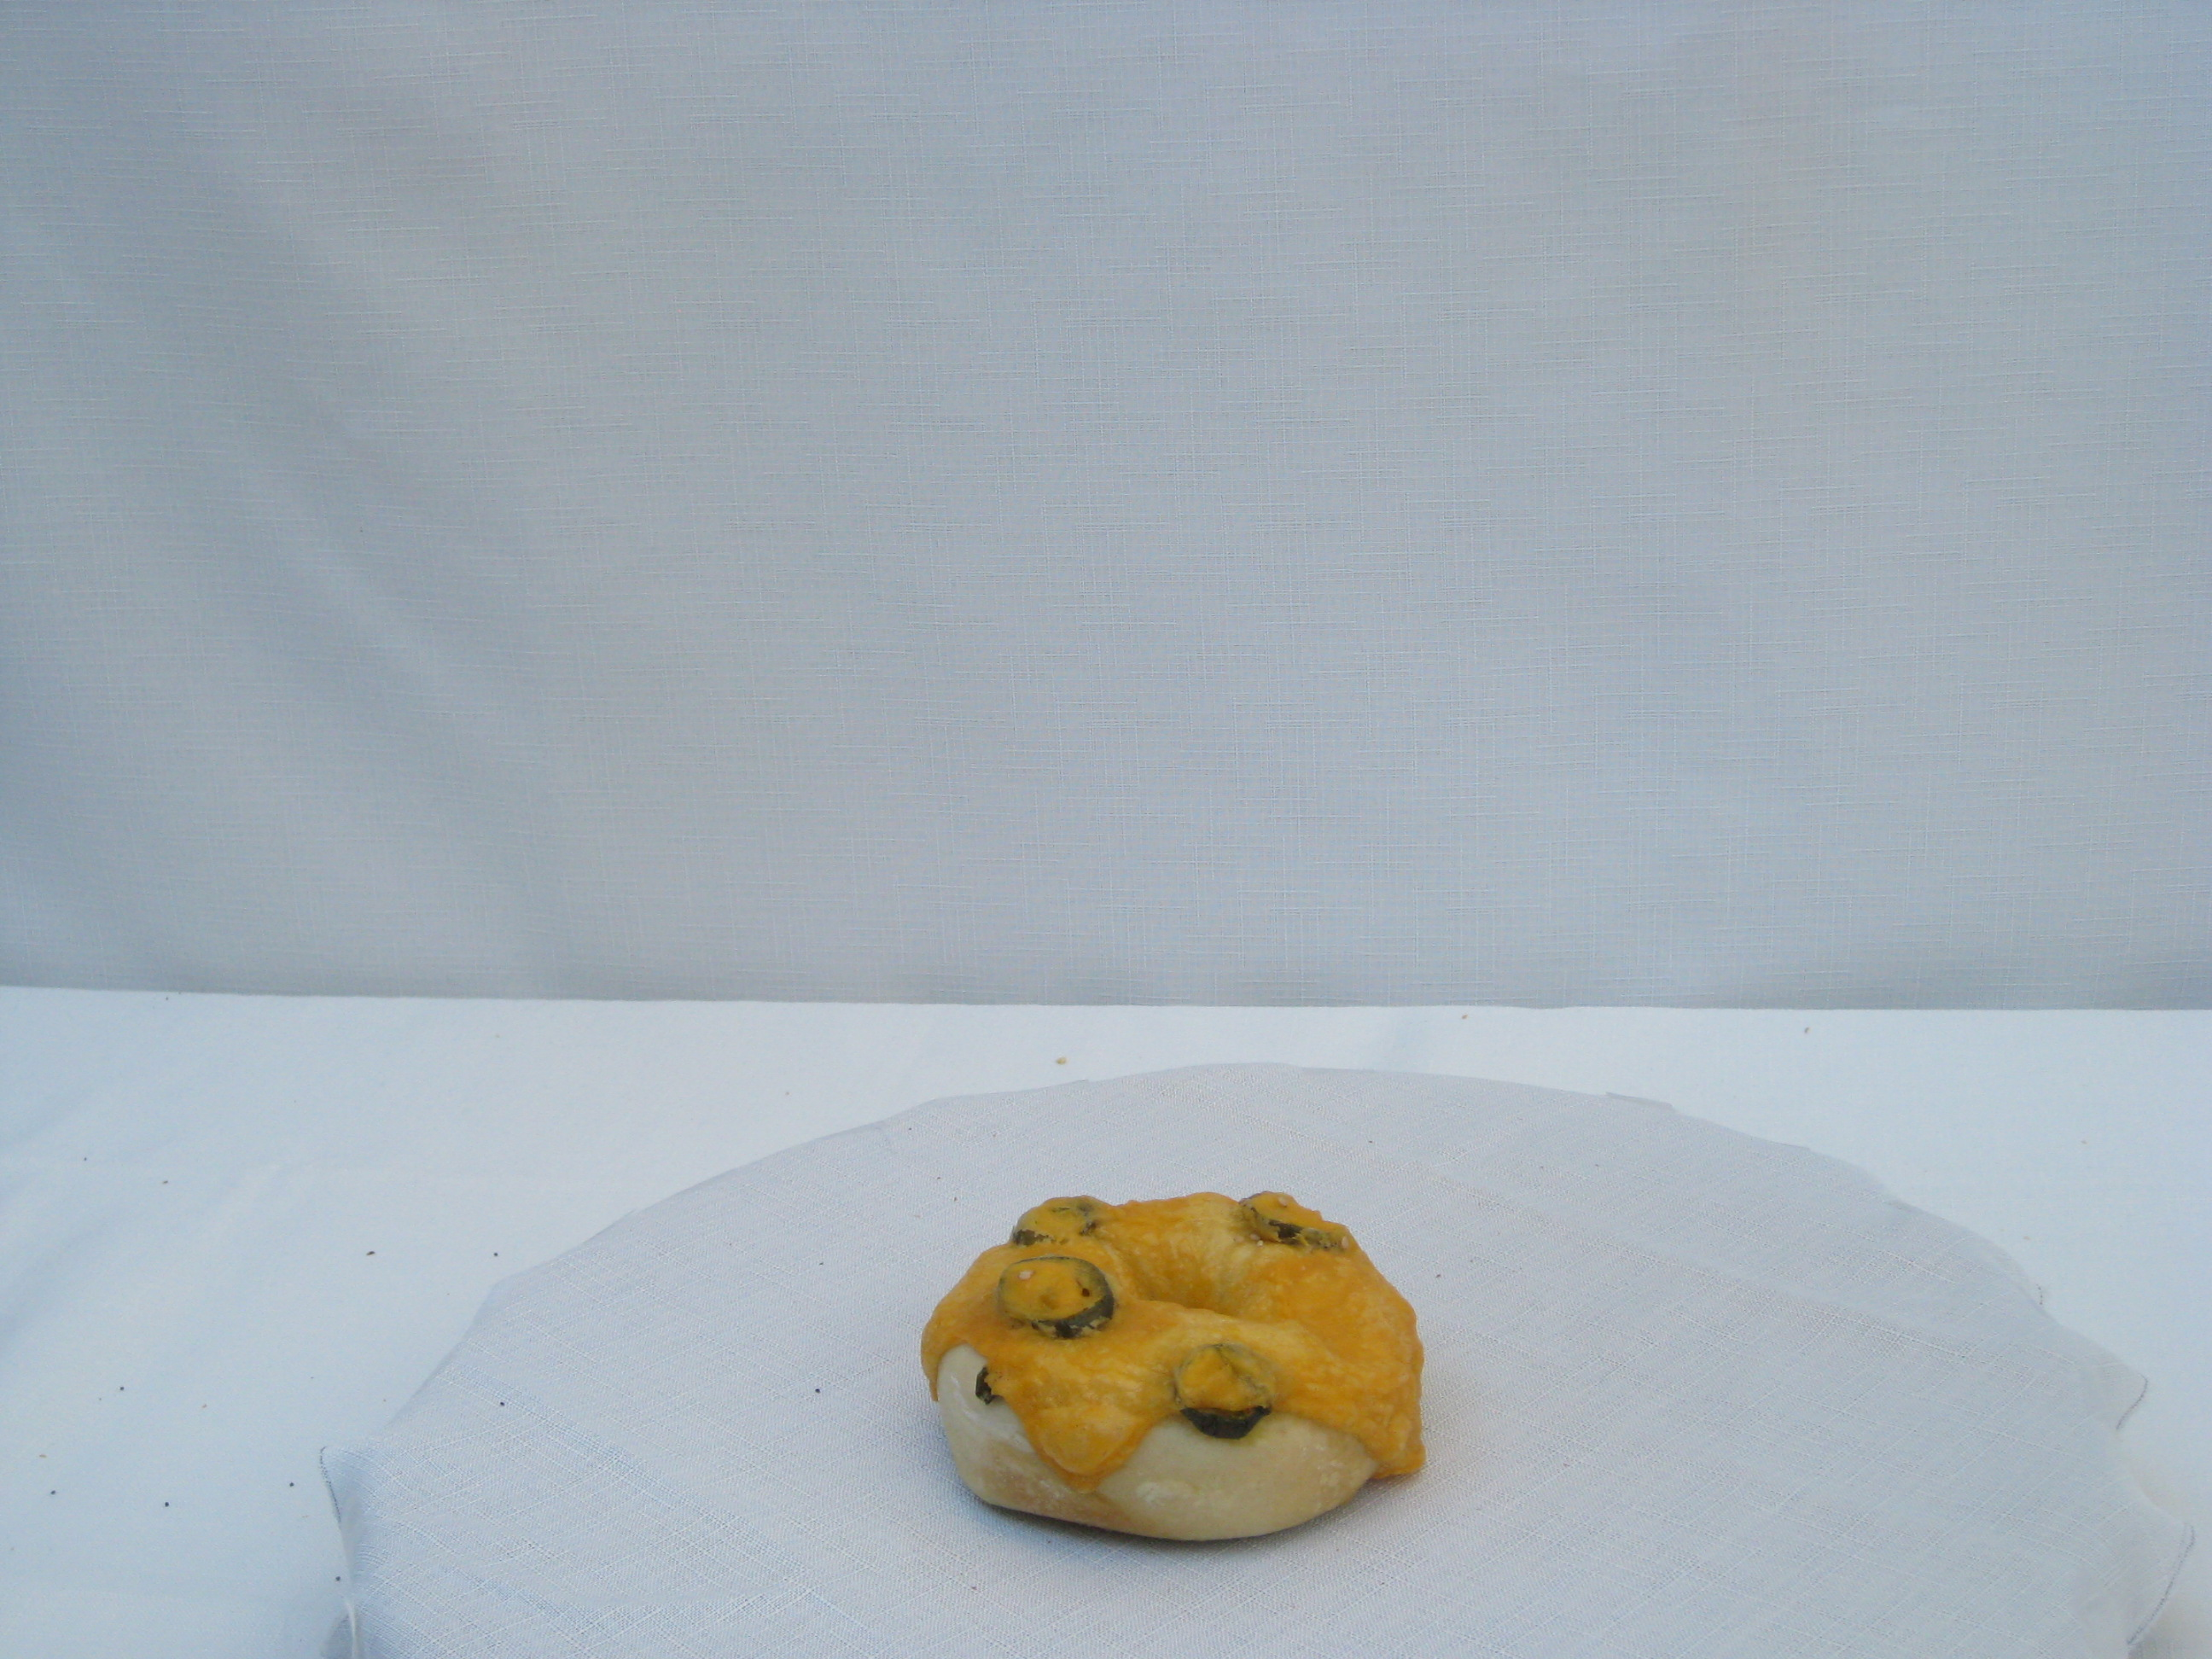
\includegraphics[width=20mm]{data/images/relWork/pfid_bagel}}
	\subfloat[doughnuts, desserts, snacks]{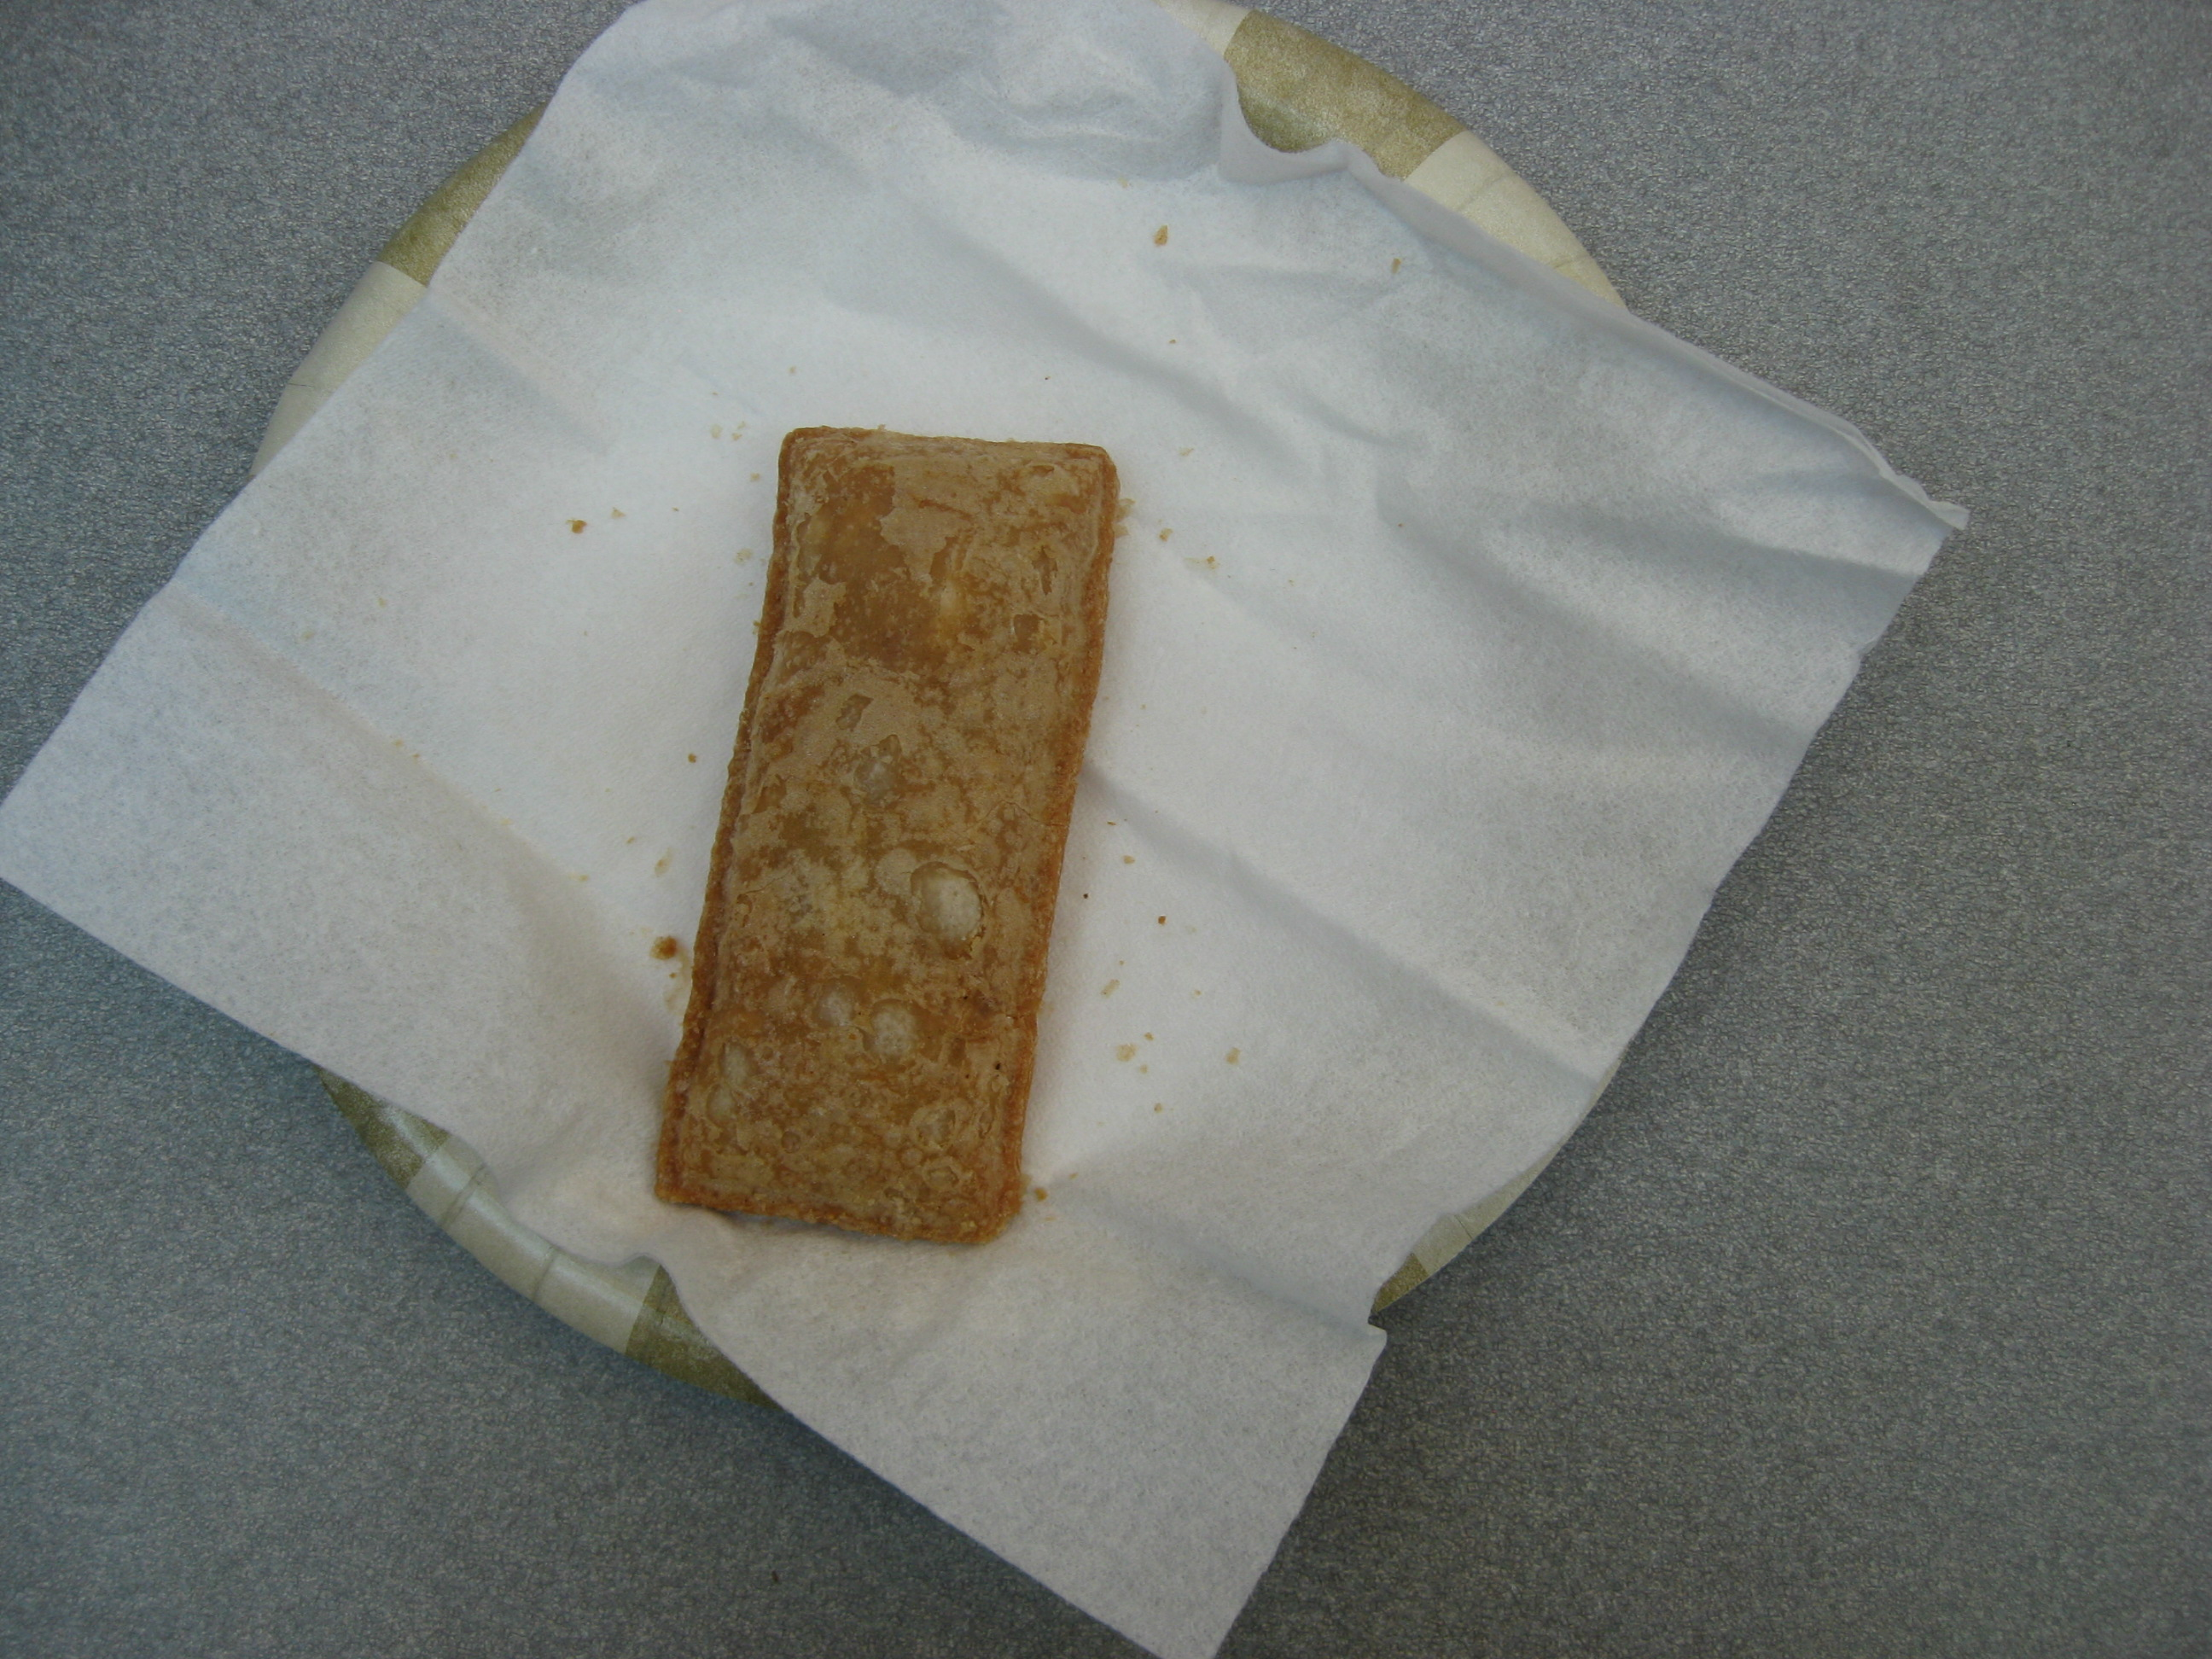
\includegraphics[width=20mm]{data/images/relWork/pfid_dessert}}
	\subfloat[pizza]{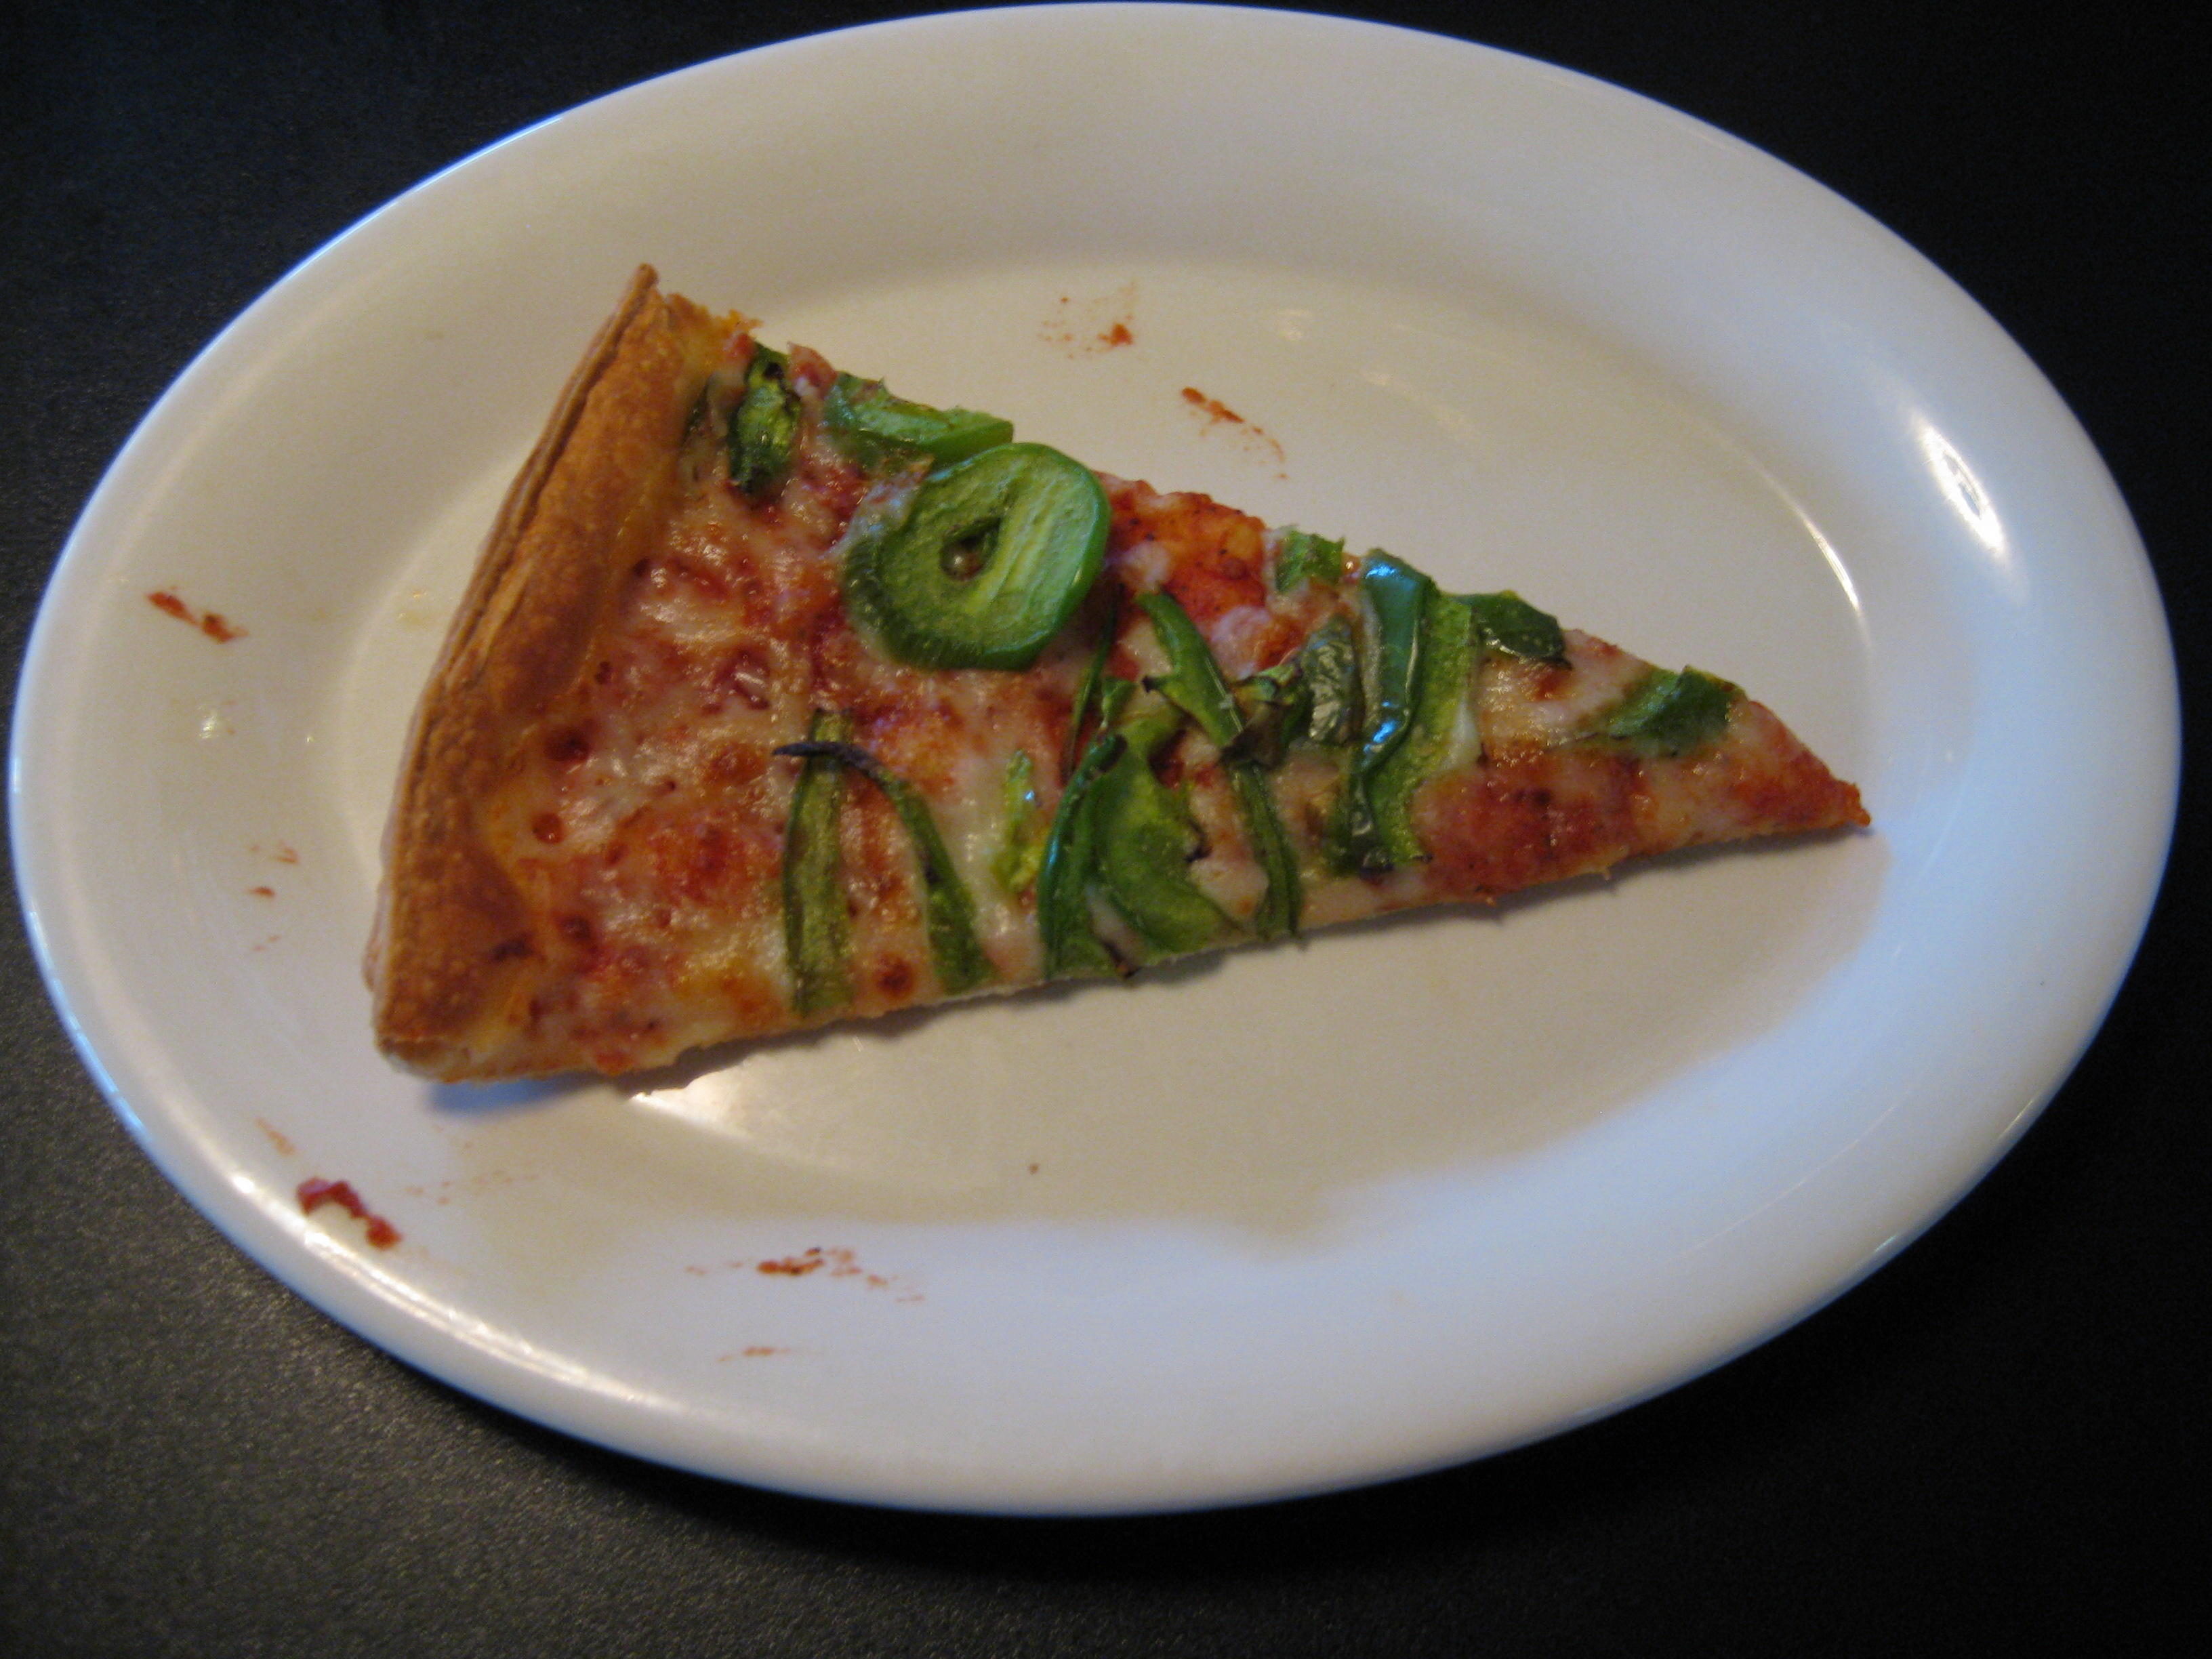
\includegraphics[width=20mm]{data/images/relWork/pfid_pizza}}
	\subfloat[misc food like soup and Mexican food]{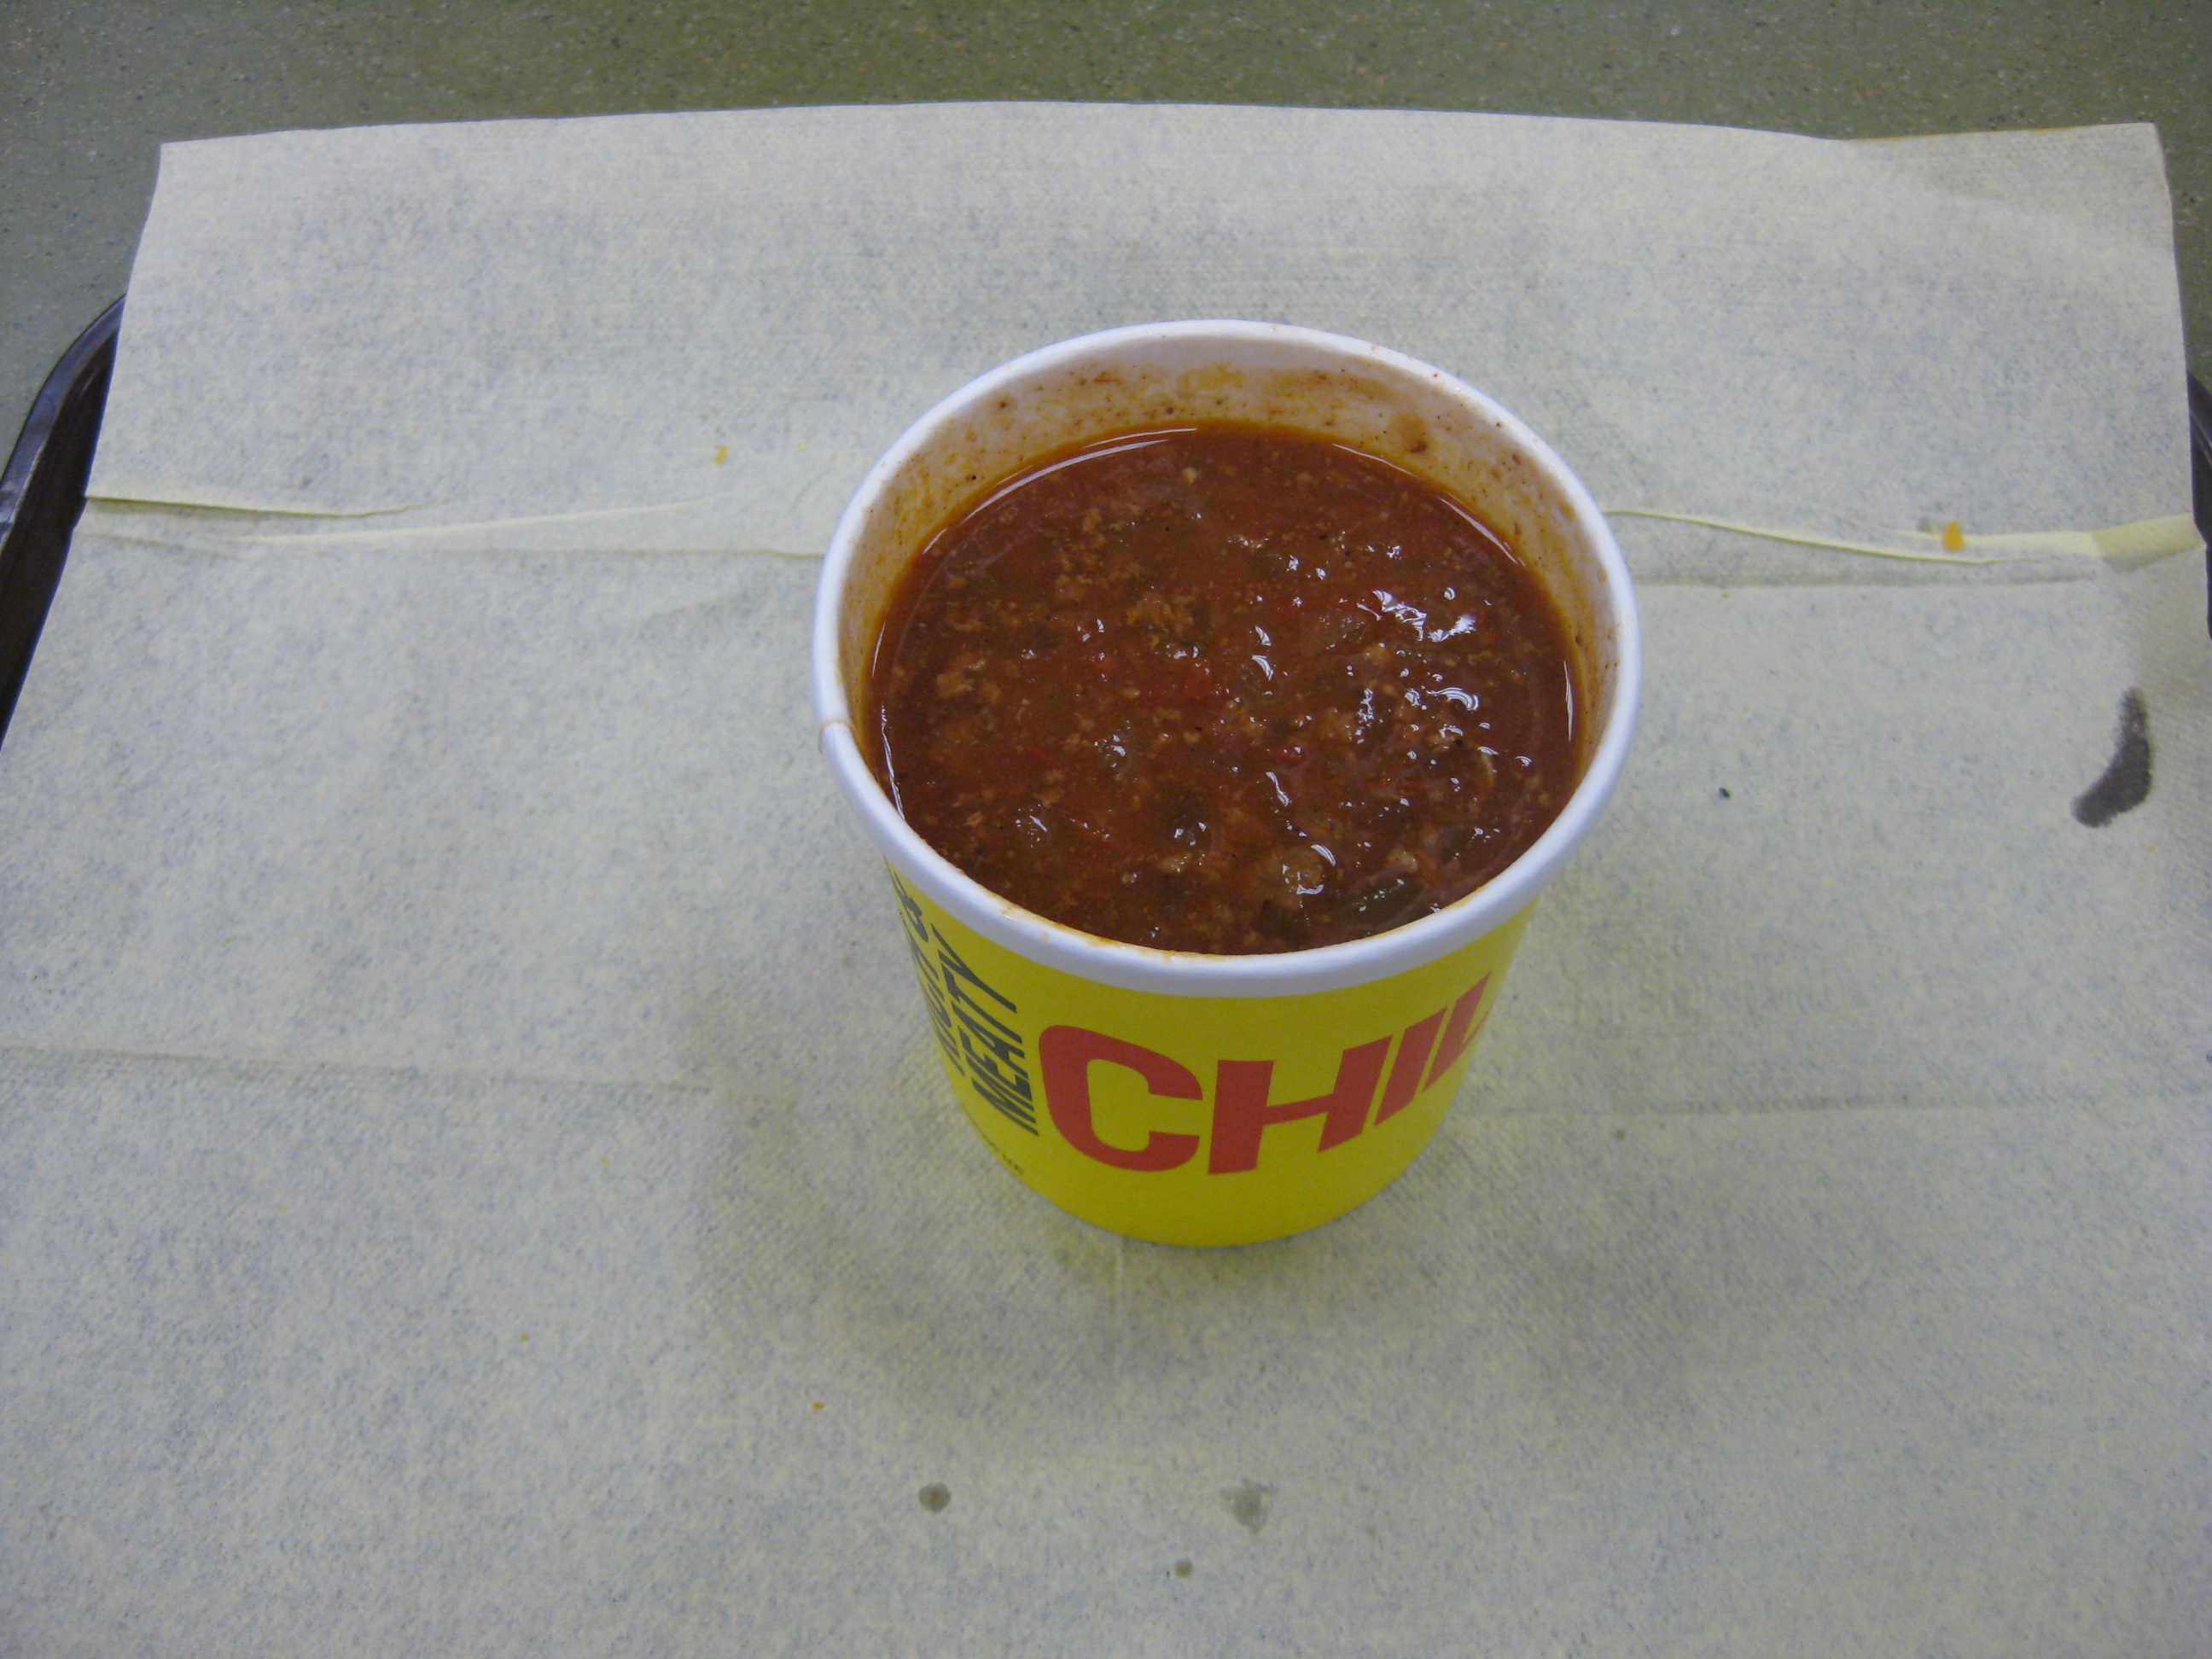
\includegraphics[width=20mm]{data/images/relWork/pfid_misc}}
	
	\caption{Examples for food items for each of the seven suggested categories in the PFID. Source: Chen et al. \cite{Chen2009}}
	\label{fig:pfidExamples}
\end{figure}

\subsection{UEC-Food-100 and UEC-Food-256}
\label{subsec:relWork_Datasets_food100256}

UEC-Food-100 \cite{Matsuda2012} and UEC-Food-256 \cite{Kawano2015} are two datasets from the \gls{uec} in Tokyo from 2012 and 2015 which were used to train "DeepFoodCam", a mobile standalone app for food classification.

The UEC-Food-100\footnote{\texttt{http://foodcam.mobi/dataset100.html}, accessed 2016-03-02} dataset comprises of 100 categories of mostly Asian cuisine. Each class contains about 100 images manually gathered from the web. Furthermore there are also bounding box information for all images. In the context of this dataset bounding boxes are very helpful for training because it is quite common in Asian countries to have several different plates of foods as shown in figure \ref{fig:food100Examples}d. The rice is only a very small part of the image and removing the other plates does significantly improve recognition performance.

With the UEC-Food-256\footnote{\texttt{http://foodcam.mobi/dataset256.html}, accessed 2016-03-02} dataset Kawano et al. increased the number of categories from 100 to 256. To collect the new data from web sources they used their original UEC-Food-100 dataset to train \glspl{svm} that calculate "foodness", a value that measures if a picture is a food item or not. Images with a high "foodness" might be food but they might not correspond to any of the new categories of  UEC-Food-256. To filter these images they applied transfer learning by selecting images with a high "foodness" value and visually similar classes from UEC-Food-100. Lastly, Kawano et al. used \gls{atm} for crowd sourcing to evaluate the results, remove remaining noise and get bounding boxes for the food items. 

\begin{figure}[htbp]
	\centering
	\subfloat[burger]{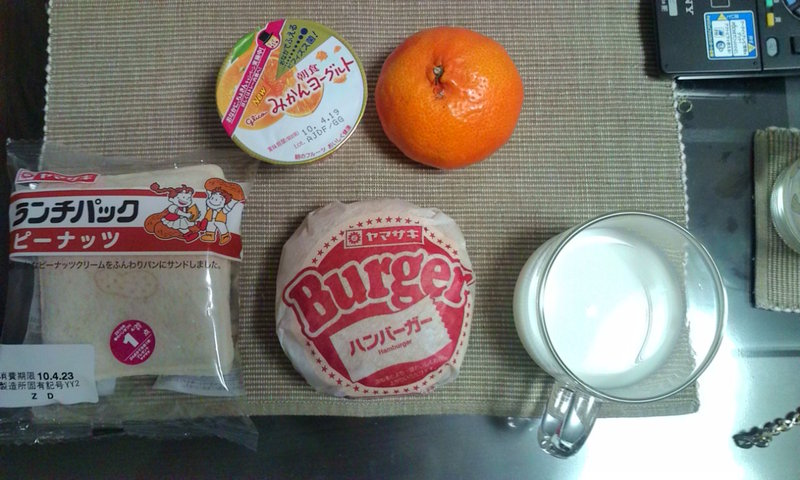
\includegraphics[width=20mm]{data/images/relWork/food100_burger}}
	\subfloat[croquette]{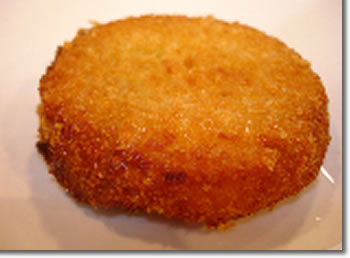
\includegraphics[width=20mm]{data/images/relWork/food100_croquette}}
	\subfloat[dipping noodles]{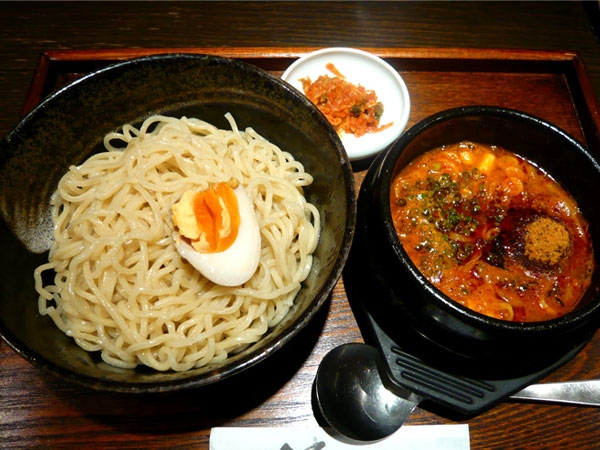
\includegraphics[width=20mm]{data/images/relWork/food100_dippingNoodles}}
	\subfloat[rice]{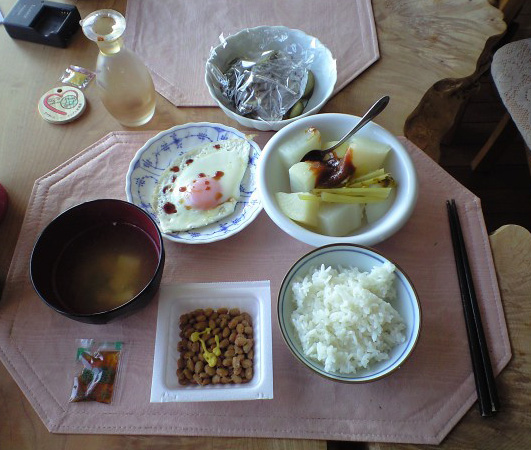
\includegraphics[width=20mm]{data/images/relWork/food100_rice}}
	\subfloat[shrimp with chill source]{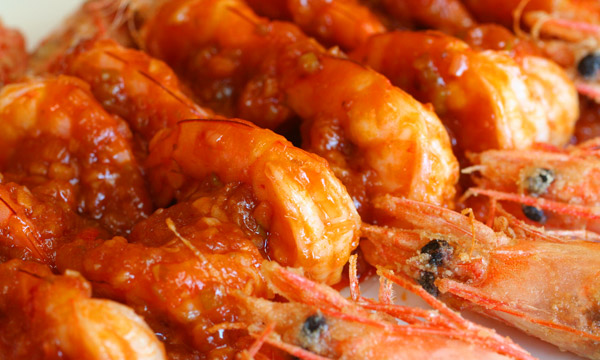
\includegraphics[width=20mm]{data/images/relWork/food100_shrimpChillSouce}}
	\subfloat[simmered pork]{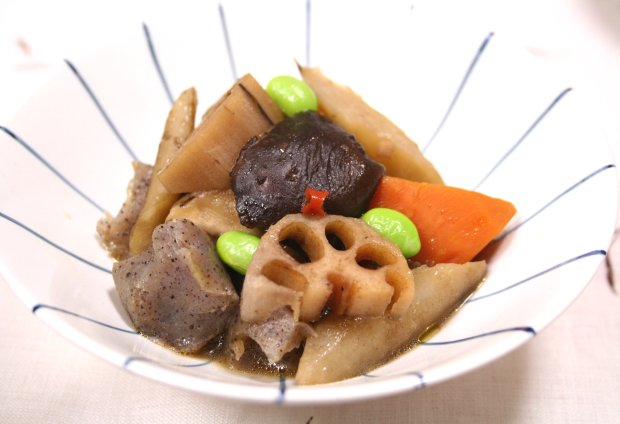
\includegraphics[width=20mm]{data/images/relWork/food100_simmeredPork}}
	\subfloat[toast]{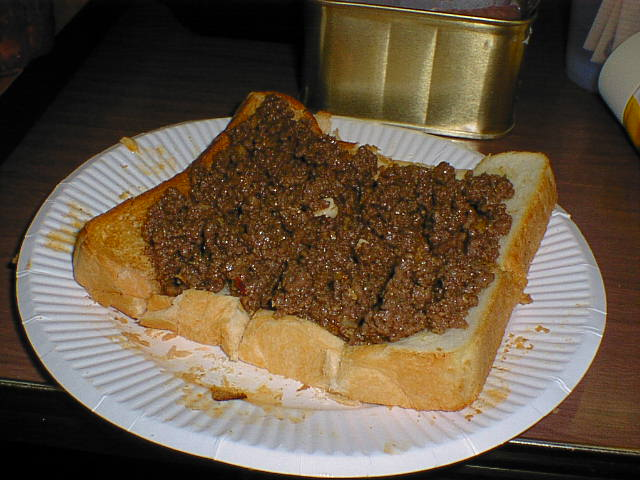
\includegraphics[width=20mm]{data/images/relWork/food100_toast}}
	
	\caption{A sample of the food items and categories of the UEC-Food-100 dataset. Source Matsuda et al. \cite{Matsuda2012}}
	\label{fig:food100Examples}
\end{figure}

\subsection{Food-101}
\label{subsec:relWork_Datasets_food101}
Food-101 is the largest food dataset so far. The original Food-101\footnote{\texttt{http://www.vision.ee.ethz.ch/datasets/food-101/}, accessed 2016-03-02} dataset was built by Bossard et al. in 2014 to create the first food dataset with more than 100 images per class \cite{Bossard2014}. They composed a list of the 101 most common keywords on \href{http://Foodspotting.com}{Foodspotting.com}. For each keyword they obtained 1000 images from the site. Figure \ref{fig:food101Examples} gives some examples of the images in the dataset. Contrary to other food datasets like \hyperref[subsec:relWork_Datasets_food100256]{UEC Food 256}, they did not remove any noise from the dataset which results in many false positive labels as figure \ref{fig:food101Noise} shows.

\begin{figure}[htbp]
	\centering
	\subfloat[French fries]{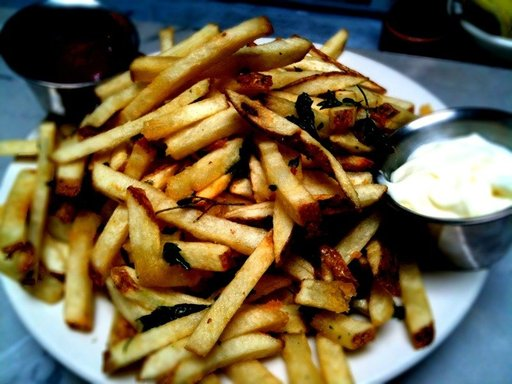
\includegraphics[width=20mm]{data/images/relWork/Efood101_frenchFries}}
	\subfloat[fried rice]{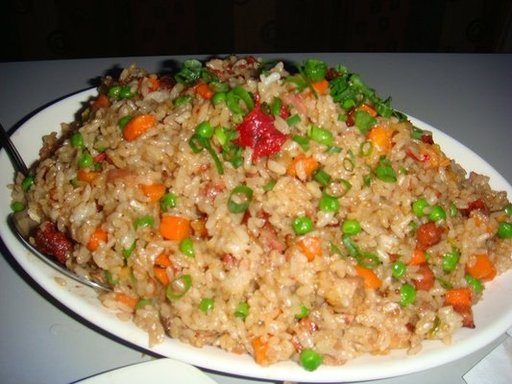
\includegraphics[width=20mm]{data/images/relWork/Efood101_friedRice}}
	\subfloat[hamburger]{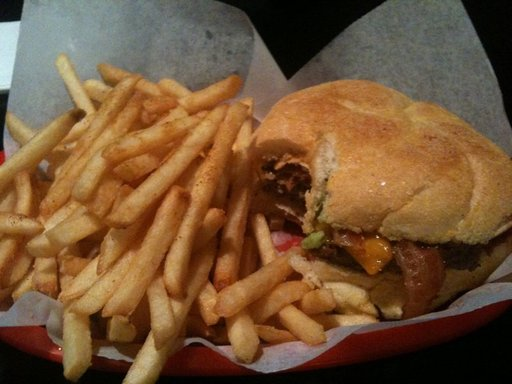
\includegraphics[width=20mm]{data/images/relWork/Efood101_hamburger}}
	\subfloat[pizza]{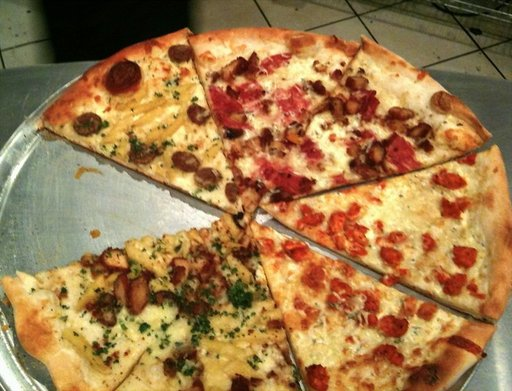
\includegraphics[width=20mm]{data/images/relWork/Efood101_pizza}}
	\subfloat[sashimi]{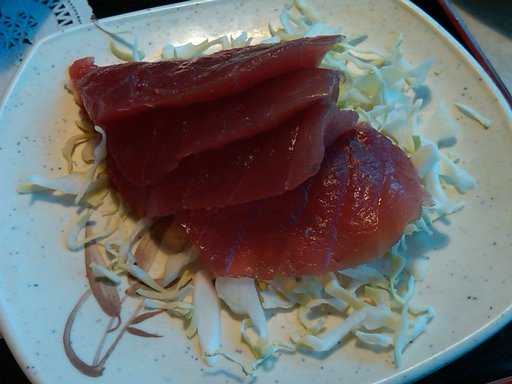
\includegraphics[width=20mm]{data/images/relWork/Efood101_sashimi}}
	\subfloat[spagetti]{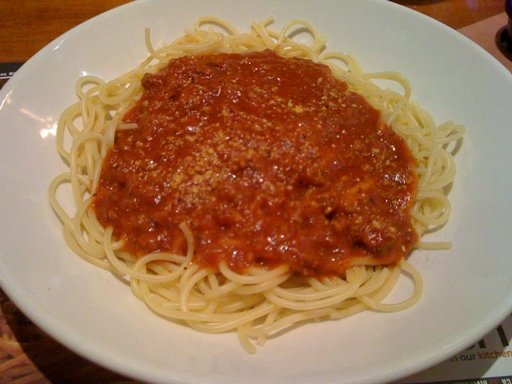
\includegraphics[width=20mm]{data/images/relWork/Efood101_spagetti}}
	\subfloat[steak]{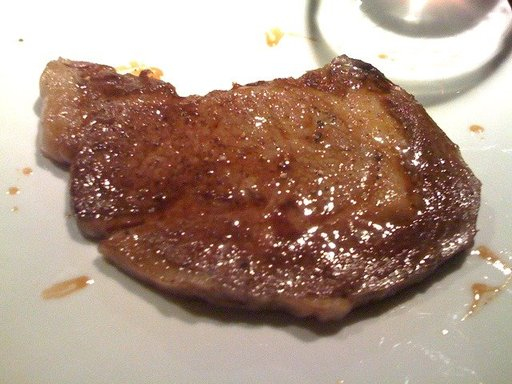
\includegraphics[width=20mm]{data/images/relWork/Efood101_steak}}
	
	\caption{A sample of the food items and categories of the ETHZ-Food-101 dataset. Source: Bossard et al. \cite{Bossard2014}}
	\label{fig:food101Examples}
\end{figure}

A year later in 2015 Kumar et al. released the UPMC-Food-101\footnote{\texttt{http://visiir.lip6.fr/explore}, accessed 2016-03-02} dataset which contains the exact same categories as the first Food-101 dataset from the \gls{ethz}. This makes it possible to combine these twin datasets into one big dataset since they contain images from different sources. The data of UPMC-Food-101 originates from Google Image search followed by the keyword "recipe" to reduce noise because some words can be associated with non-food-items {(eg. Hamburger-menu-icon, escargots as living snails)}. However, despite the keyword "recipe" UPMC-Food-101 contains even more noise than ETHZ-Food-101. Additionally, for 100,000 images, they included the \gls{html} of the pages the images were embedded in \cite{Kumar2015}. 

\begin{figure}[htbp]
	\centering
	\subfloat[French fries]{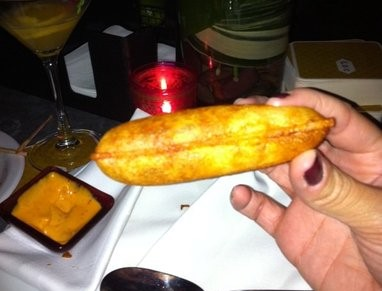
\includegraphics[width=20mm]{data/images/relWork/Nfood101_frenchFries}}
	\subfloat[fried rice]{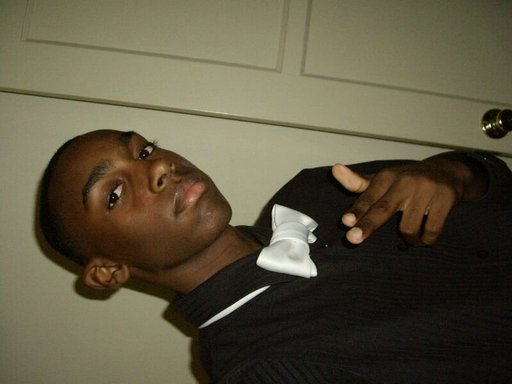
\includegraphics[width=20mm]{data/images/relWork/Nfood101_friedRice}}
	\subfloat[hamburger]{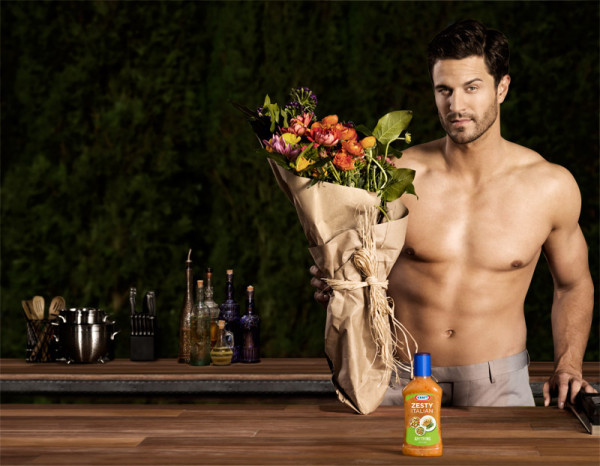
\includegraphics[width=20mm]{data/images/relWork/Nfood101_hamburger}}
	\subfloat[pizza]{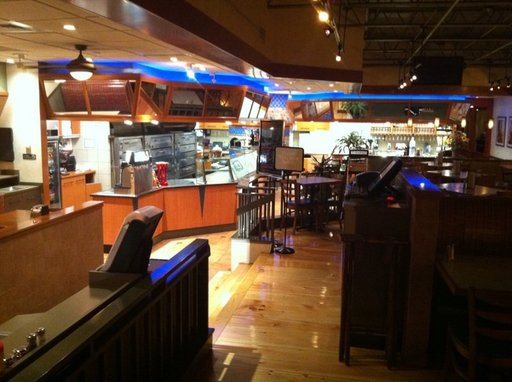
\includegraphics[width=20mm]{data/images/relWork/Nfood101_pizza}}
	\subfloat[sashimi]{
\includegraphics[width=20mm]{data/images/relWork/Nfood101_sashimi}}
	\subfloat[spagetti]{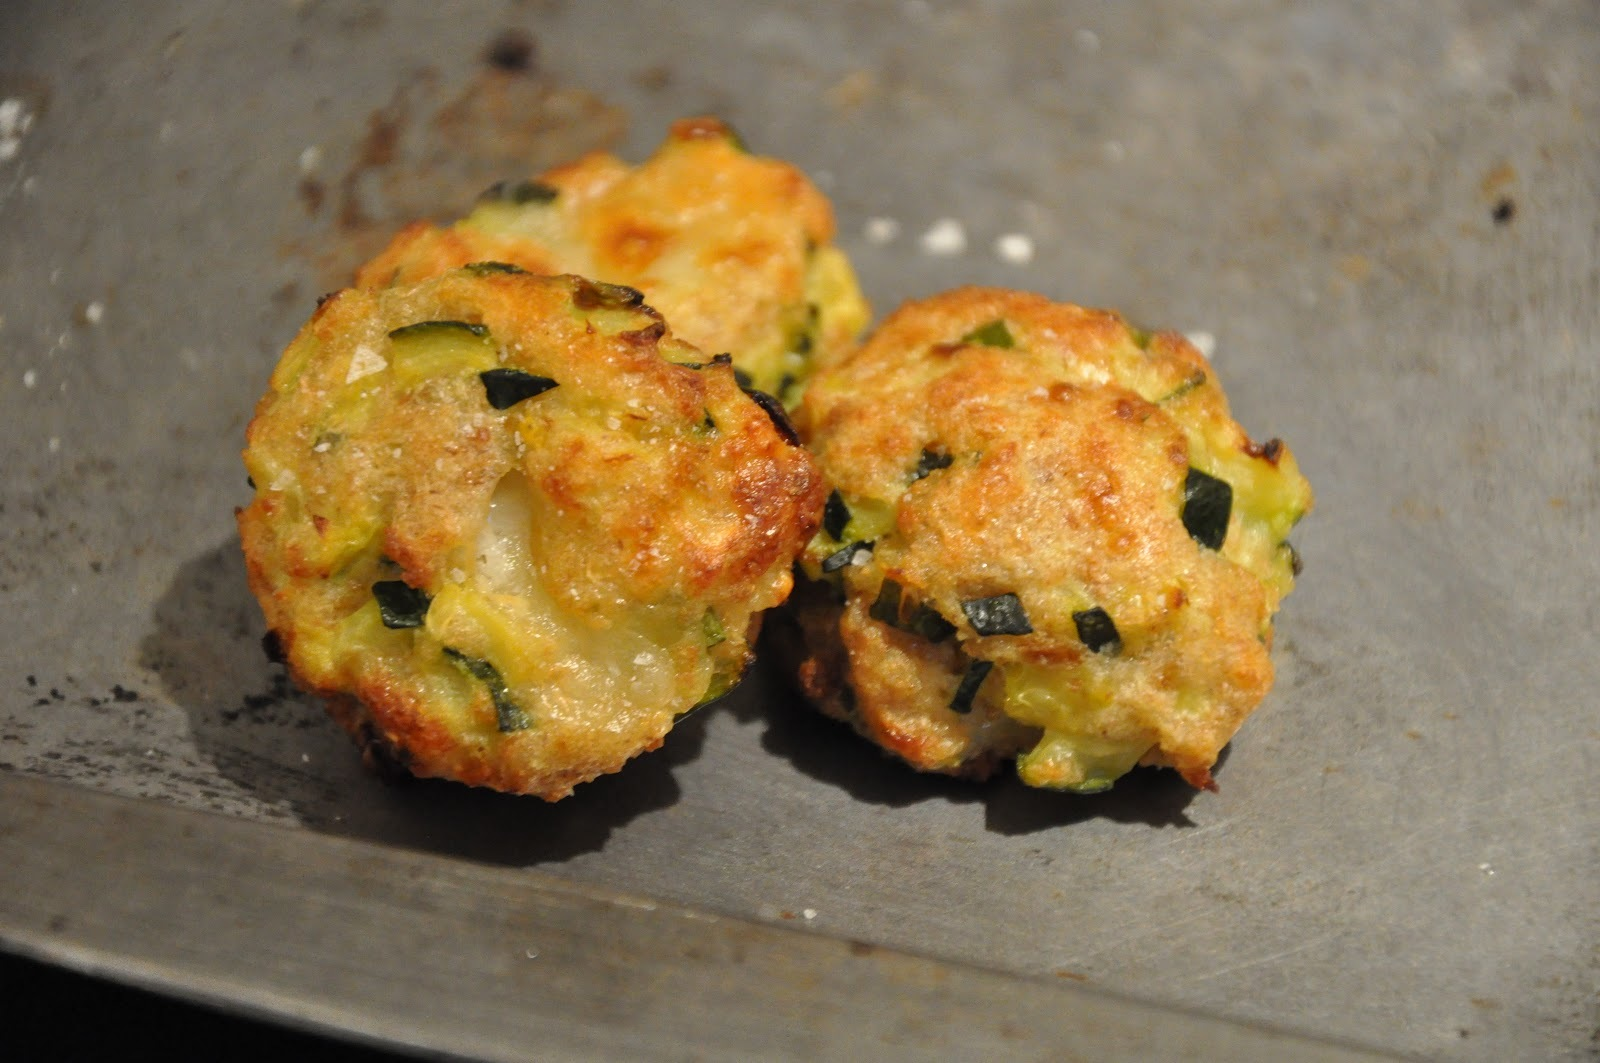
\includegraphics[width=20mm]{data/images/relWork/Nfood101_spagetti}}
	\subfloat[steak]{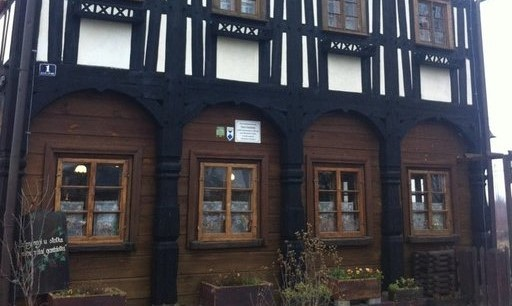
\includegraphics[width=20mm]{data/images/relWork/Nfood101_steak}}
	
	\caption{Examples for noise in the Food-101 datasets. Source: Kumar et al. \cite{Kumar2015} and Bossard et al. \cite{Bossard2014}}
	\label{fig:food101Noise}
\end{figure}

\subsection{Food-201}
\label{subsec:relWork_Datasets_food201}
With the upcoming Food201 datasets Meyers et al. are trying to address several shortcomings of the Food-101 datasets \cite{Meyers2015}. Food201-MultiLabel will be a subset of the original ETHZ-Food-101 dataset containing only 50\% of the images. They took 47,374 of those images to \gls{atm} to label the contents of the images individually since a major problem of Food-101 is the lack of multiple labels for images as demonstrated in figure \ref{fig:food101Examples}c. A picture could contain some French fries and a burger but might be only labeled in the category of Burger. Even if a classifier correctly predicts "french fries" as a possible solution for the problem the result will still be marked as incorrect. The new dataset now contains 201 categories in contrast to the 101 previously with a mean of 1.9 different labels per image.

Food201-Segmented will be another smaller subset of Food201-MultiLabel with 12,625 images and pixelwise labeling of the category. This dataset will enable a better training of segmentation oriented classifiers.

At this point in time the Food201 datasets are not released\footnote{\texttt{https://storage.googleapis.com/food201/food201.zip}, accessed 2016-03-02}.

\subsection{ImageNet}
\label{subsec:relWork_Datasets_imgNet}
ImageNet is the biggest general image recognition dataset to this date containing 21,841 classes and 14,197,122 images \cite{Russakovsky2015}. Considering that a sizeable amount of the dataset consists of food, ImageNet could be counted as a food image recognition dataset. However, the effort one has to spend to actually get only the food data is quite high. Categories in ImageNet are organized as \glspl{synset}. \Glspl{synset} can have different children called hyponyms. The \gls{wnid} for the food \gls{synset} is \texttt{n00021265}. By using an \gls{api} call\footnote{\texttt{http://www.image-net.org/api/text/wordnet.structure.hyponym?wnid=wnid\&full=1}} and the food \gls{wnid}, ImageNet returns a list of all food-\glspl{hyponym}. With these \glspl{wnid} the image \glspl{url} can be obtained by another \gls{api} call. ImageNet contains 1527 food categories, yet, some of these categories only contain a small amount of images while others include many images making the dataset imbalanced which makes it harder to train certain classifiers like \glspl{svm} \cite{Batuwita2013}.

\subsection{Menu-Match}
\label{subsec:relWork_Datasets_menuMatch}
Despite its small size of only 646 images distributed over 41 classes, Menu-Match is an important dataset in the domain of computer vision food calorie estimation because it is the only dataset available in public\footnote{\texttt{http://research.microsoft.com/en-us/um/redmond/projects/menumatch/data/}, accessed 2016-03-03} which includes professional calorie estimations for each food \cite{Beijbom2015}. Beijbom et al. collected meals from three restaurants and made images with seven different capture devices {(six smartphones and one point and shoot camera)} in a real world scenario without fixed camera angles or distances.

\subsection{Other Smaller Food Datasets}
In addition to the mentioned food datasets there are several other notable datasets in the extended domain of food classification. Chen et al. published a small Chinese food dataset with 50 classes and 100 images per class \cite{Chen2012}. They did not give a name to the dataset so this dataset is refereed to as "50-data" is this thesis. Moreover, there are three other food datasets which belong to the extended set of food classification datasets. 
\newline\newline
\gls{tada} is a project of the Purdue University. For their project they developed an image database called I-TADA that includes images as well as meta-data \cite{Khanna2010}.
\newline\newline
\gls{frida} is a food image database with 877 images belonging to eight classes including natural-food {(e.g. fruit)}, processed food {(e.g. french fries)}, rotten-food, natural-non-food items {(e.g. pinecone)}, and classes that contain non food items \cite{Foroni2013}.
\newline\newline
Lastly, "Food.pics" is a dataset of 568 food items that was developed to asses the relevance of visual food cues for the human brain \cite{Blechert2014}. 

\section{Algorithms}
\label{sec:relWork_Algorithms}
Although food is much harder to recognize and classify than common object recognition, it is considered as a computer vision problem so most of the common computer vision and machine learning algorithms can be applied. Unfortunately, it is not easy to compare algorithms and methods of different papers based on their results. Different authors seldom use the same benchmarks and often even use their own closed source datasets which makes even basic comparison impossible. In addition, these algorithms can often be parametrized and not all papers publish all parameters so even identical algorithms can achieve different accuracies. As a result, this section will expose the algorithms and methods but not compare them. Figure \ref{fig:overviewAlgorithms} gives an overview of the different techniques used in 43 food recognition publications.

\begin{figure}[ht]
	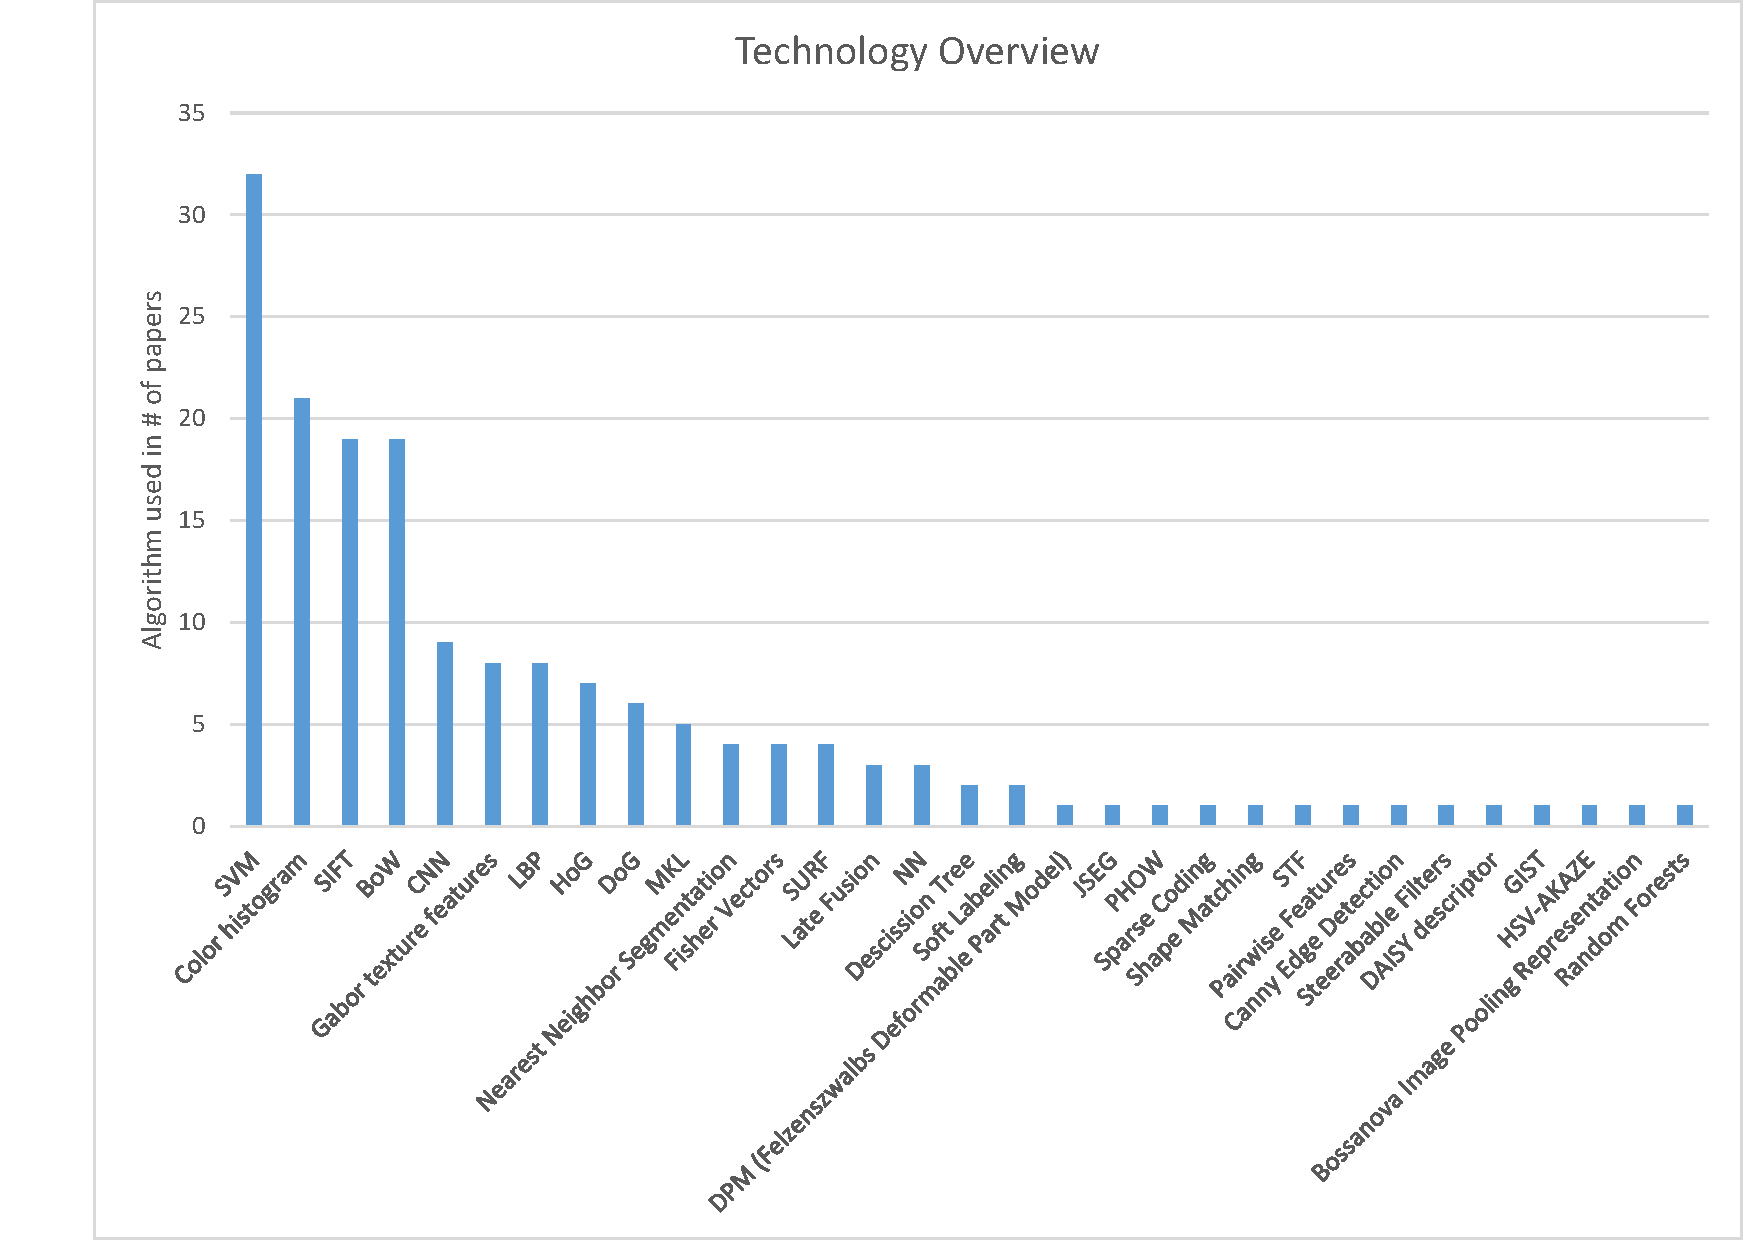
\includegraphics[width=\linewidth]{figures/technologyOverview}
	\caption{Number of occurrences of different computer vision and machine learning algorithms used in 43 papers in the domain of food recognition.}
	\label{fig:overviewAlgorithms}
\end{figure}


The most used approach for food classification in literature is still the use of various feature descriptors transformed into fixed length vectors and \gls{svm} classification. Out of 43 publications in the domain of food recognition, 72\% of these papers used a support vector machine. 

\subsection{Color Features}
In contrast to normal object recognition color features such as histograms play a much more important role for food recognition because color is one of the main characteristics of food. The color of a car does not matter but it makes a huge difference if the pasta sauce is red or white.

The use of color features for food classification can be divided into three approaches:
\begin{enumerate}
	\item Histograms
	\item First- and second moment statistical values
	\item Color descriptors
\end{enumerate}

Since using approaches {(1)} or {(2)} means neglecting any spatial relations most publications sub divide the images into 2x2 \cite{Joutou2009, Hoashi2010, Kawano2014a} or 4x4 blocks \cite{Chen2012} and apply the algorithms separately to keep basic spatial relations.

\subsubsection*{{(1)} Histograms}
The most common color histogram feature is a 64 bin \gls{rgb} histogram \cite{Joutou2009, Hoashi2010, Chen2009}. Prabu tested five different histograms based on the color space and normalization but didn't provide any results in his paper \cite{Prabu2015}.

\subsubsection*{{(2)} First- and second moment statistical values}
There are several possible values that can be utilized to create a meaningful feature vector such as mean of pixel values in different color spaces \cite{Kitamura2008, Kim2010, Kawano2014a, Bosch2014} or variance / deviation \cite{Kitamura2008, Kawano2014a, Bosch2014}. Bosch et al. also used the most dominant color in a block as an additional value \cite{Bosch2014}.

\subsubsection*{{(3)} Color descriptors}
The performance of primitive color features like {(1)} and {(2)} can suffer greatly from changes in the environment like illumination changes. Therefore, recent publications used colour descriptors instead of histograms or statistical measurements \cite{Beijbom2015, Bettadapura2015}.

\subsection{Feature Detectors and Descriptors}
Following color features, \gls{sift} \cite{Lowe1999} is the most used feature detector and descriptor. Out of 43 publications, 21 used \gls{sift} to classify food \cite{Kitamura2009, Joutou2009, Wen2009, Chen2009, Kitamura2010, Zong2010, Hoashi2010, Chen2012, Kim2014, Farinella2014, Nguyen2014, Bosch2014, Kagaya2015, Kumar2015, Prabu2015, Beijbom2015, Bettadapura2015, Probst2015}. Unfortunately, there is no paper with a comparison between different numbers of \gls{sift} keypoints or parameters for food recognition.

\gls{sift} is often used in combination with a \gls{bow} \cite{Joutou2009, Chen2009, Kitamura2010, Zong2010, Hoashi2010, Chen2012, Matsuda2012, Kim2014, Nguyen2014, Bosch2014, Kagaya2015, Kumar2015, Beijbom2015, Probst2015}. For \glspl{bow}, according to Joutou et al., a higher \gls{bow} codebook dimension of 2000 is better than a lower dimension of 1000 \cite{Joutou2009}.

Other popular image features include \gls{hog} \cite{Puri2010, Hoashi2010, Matsuda2012, Kim2014, Kawano2014, Kajiwara2015, Beijbom2015} and Gabor textures \cite{Joutou2009, Boushey2010, Hoashi2010, Kim2010, Matsuda2012, Kajiwara2015, Chen2012, Ponrani2014, Bosch2014} but in comparison to other image features they do not achieve high accuracies \cite{Kim2014, Beijbom2015}. Hoashi et al. compared several \gls{hog} classifiers to Gabor filters and \glspl{bow}. Even a \gls{bow} with random keypoint sampling achieved a better result {(30.35\%)} than the best \gls{hog}- or Gabor classifiers {(21.84\% and 25.35\%)} \cite{Hoashi2010}.

Publications also made use of \gls{lbp} \cite{Zong2010, Chen2012, Christodoulidis2015, Prabu2015, Beijbom2015}. Farinella et al. tested \gls{pricolbp}, a slightly different \gls{lbp} algorithm which outperformed \gls{sift} \cite{Farinella2014} and Nguyen et al. compared \gls{lbp} and \gls{nrlbp} with \gls{nrlbp} achieving marginally better results than normal \gls{lbp}. 


\subsection{Convolutional Neural Networks}
Recent approaches showed that deep learning can produce much higher accuracies than the classical feature and \gls{svm} combinations.

Kim was one of the first to use a \gls{cnn} for food recognition but only achieved 22.38\% of accuracy on the \hyperref[subsec:relWork_Datasets_food100256]{UEC-Food-100} dataset due to the lack of images because UEC-Food-100 only contains about 100 images per class \cite{Kim2014}. Therefore, his proposed \gls{phow} approach achieved a much higher accuracy with 32.12\%.

Kawano et al. used a slightly different approach on UEC-Food-100 \cite{Kawano2014}. They took a modified 8-layer-\gls{cnn} which was pretrained on the \gls{ilsvrc} 1000 class dataset. They removed the last layer {(layer 8)} and utilized the output of layer 7 as a feature vector which was then used in combination with Fisher vectors to classify the image. With this \gls{cnn} they outperformed every other result on UEC-Food-100 with an accuracy of 72.26\%. Their second \gls{cnn} got even better results. It was a \gls{cnn} pretrained on the \gls{ilsvrc} 2000 class dataset which they further enhanced by using 1000 food-\glspl{synset} from ImageNet. This more food related \gls{cnn} could achieve an accuracy of 77.35\%.

Kumar et al. used a very similar approach in their publication \cite{Kumar2015}. They also used the output of the layer before the last layer as a feature vector and they also used a pretrained net.

Bossard et al. trained the \gls{cnn} which Krizhevsky originally proposed in \cite{Krizhevsky2012} {(AlexNet)}. They used this net as a baseline for their new \hyperref[subsec:relWork_Datasets_food101]{Food-101} dataset and got a result of 56.40\% \cite{Bossard2014}.

Kagaya et al. tested different architectures of small \glspl{cnn} against their own closed source "FoodLog" dataset with 10 classes \cite{Kagaya2015}. With 73.70\% they achieved the best result by using a two layer network with small 5x5 kernels.

Christodoulidis and Anthimopoulos also compared different smaller CNN architectures on their own dataset with 7 different classes and got the best results (71.79\%) with a 6-layer CNN that used dropout \cite{Christodoulidis2015}.

Shimoda and Yanai used a pretrained AlexNet \gls{cnn} to segment images of the UEC-Food100 dataset into different components \cite{Shimoda2015}.

Myers et al. recently released a paper for their "Im2Calories" system which almost solely relies on \glspl{cnn} \cite{Meyers2015}. Like other approaches they utilize \glspl{cnn} which are trained on ImageNet. In this case they took a GoogLeNet \gls{cnn}, replaced the last layer with a 101-way softmax layer and trained the net on Food-101. The reported 79\% accuracy is much better than the previous benchmark for Food-101 with 50.76\%. They also used \glspl{cnn} for automatic food segmentation and volume estimation. For the segmentation task they used "DeepLab", a \gls{cnn} in combination with a \gls{crf} from \cite{Chen2014}. This method and additional context information accomplished a top-1 accuracy of 76\% on their \hyperref[subsec:relWork_Datasets_food201]{Food201-Segmented} dataset. For the volume estimation they used the network from \cite{Eigen2015} and got an average relative error of 0.18 meters.


\section{Existing Systems}
\label{sec:relWork_exSystems}
The following section includes three existing systems. One of them is already available estimating food groups. There are also two other systems that are not publicly available but include calorie estimation.

\subsection{FoodLog}
\begin{figure}[htbp]
	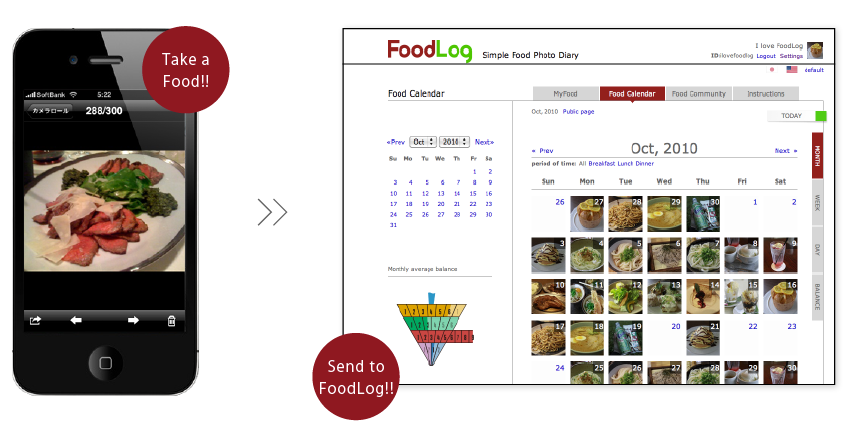
\includegraphics[width=\linewidth]{data/images/relWork/foodLog_screenshot}
	\caption{Image of the FoodLog system taken from the website. Source: \cite{Inc.}.}
	\label{fig:foodLogScreenshot}
\end{figure}

FoodLog\footnote{\texttt{http://www.foodlog.jp/en/}, accessed 2016-03-07} is a online webservice by researches from the University of Tokyo that has been online since march 2009 \cite{Kitamura2008, Kitamura2009, Kitamura2010}. This service allows users to record their daily food intake with photos to support diets and weight loss. FoodLog analyzes the submitted photos and verifies that the uploaded image contains food. If an image contains food the service calculates the "food balance" which is the share of five food groups {(Grain, Vegetable, Meat + Beans, Dairy Products, Fruit)}. FoodLog analyzes the images using both global features like Hough transforms and color statistics and local features like \gls{sift}. Their current best result for their food balance classifier is 43\% \cite{Kitamura2010}.

\subsection{Menu-Match}
"Menue-Match" by Beijbom et al. \cite{Beijbom2015} is a collaboration between Microsoft and the University of California . They proposed a system that works exclusively on restaurant menu items and tries to estimate the amount of calories in a meal. By restricting the application to restaurants they can utilize the phone's \gls{gps} sensor to get the current position and restaurant. Knowing the restaurant's menu they can then use the menu as additional context information. The system uses five image features and a one-vs-rest linear \gls{svm} for each feature and each food class resulting in a 205 dimensional feature vector which is then trained for each image on other \glspl{svm}. This joint-feature-late-fusion approach achieved a mean absolute calorie estimation error of 232 calories per meal. At this point in time there are no apparent plans to release Menu-Match to the public. 

\subsection{Im2Calories}
\begin{figure}[htbp]
	\centering
	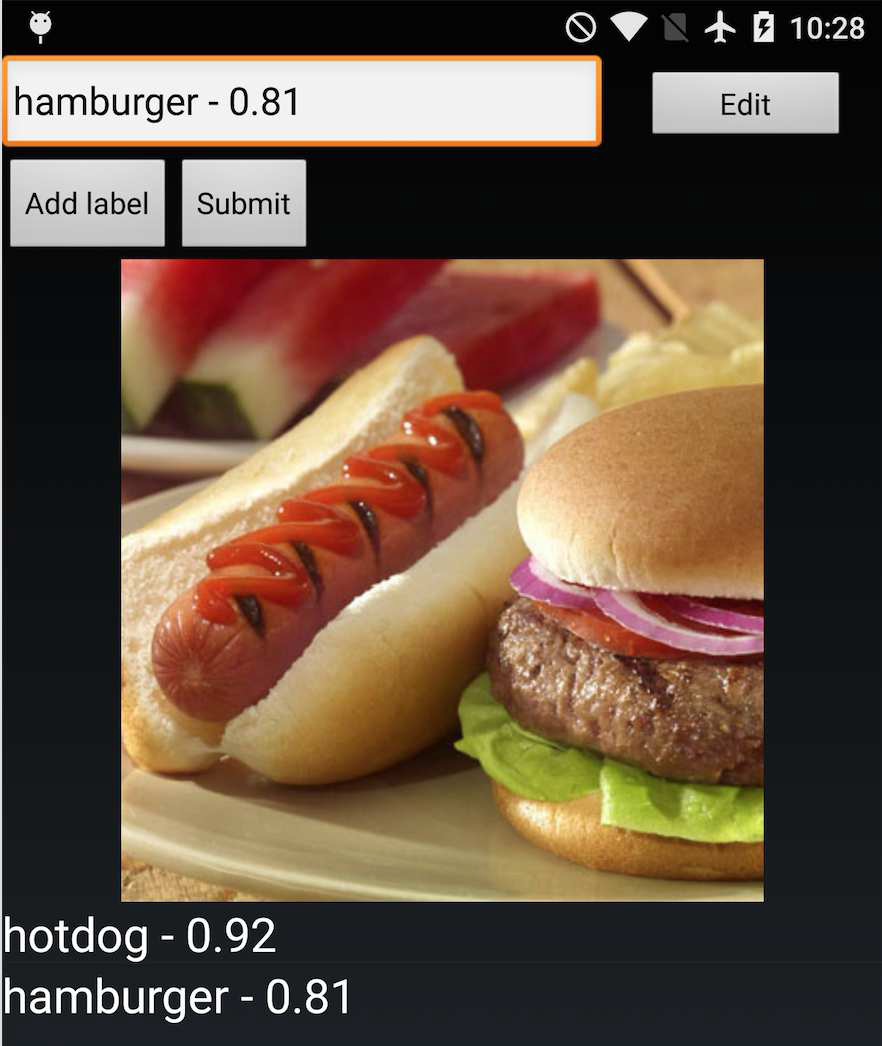
\includegraphics[scale=0.25]{data/images/relWork/im2calories_screenshot}
	\caption{Screenshot of the Image2Calories mobile Android. Source: Myers et al. \cite{Meyers2015}}
	\label{fig:im2caloriesScreenshot}
\end{figure}
Im2Calories by Myers et al. \cite{Meyers2015} is Google's approach for a computer vision aided food calorie estimator. The proposed system is similar to Menue-Match. It also tries to estimate nutritional information from food and they also set their focus on restaurant meals. However, Im2Calories tries to take it a step further. They extend the number of restaurants from 3 to 23 and instead of 41 food items they try to recognize 2517 food items. By using a deep learning approach instead of \glspl{svm} {(more details in Section \ref{sec:relWork_Algorithms})} they could improve the mean absolute calorie estimation error from 232.0 calories to 152.95. They created an Android mobile app which can classify images without an internet connection by storing the \gls{cnn} models on the device itself. A screenshot of the app can be seen in figure \ref{fig:im2caloriesScreenshot}. Google plans to release Im2Calories but has given no release date as of now. 